\documentclass[10pt,twocolumn]{article}

%% ─── Packages ─────────────────────────────────────────────────────────────────
\usepackage[margin=0.72in,columnsep=0.26in,top=0.80in,bottom=0.80in]{geometry}
\usepackage[T1]{fontenc}
\usepackage[utf8]{inputenc}
%% mathptmx removed — causes rsfs10 font errors in BasicTeX
\usepackage{amsmath,amssymb,amsfonts}
\usepackage{graphicx}
\usepackage{booktabs}
\usepackage{tabularx}
\newcolumntype{L}{>{\raggedright\arraybackslash}X}  %% auto-width wrapping column
\usepackage[font=small,labelfont=bf,skip=4pt]{caption}
%% microtype removed — requires scalable fonts not available in BasicTeX
\usepackage{xcolor}
\usepackage{url}
\usepackage{fancyhdr}
%% enumitem removed — not available in BasicTeX/TeX Live Basic
\usepackage{listings}
\usepackage[normalem]{ulem}     %% for \sout if needed
\usepackage{hyperref}
\definecolor{linkblue}{RGB}{25,85,155}
\hypersetup{
  colorlinks = true,
  linkcolor  = linkblue,
  citecolor  = linkblue,
  urlcolor   = linkblue,
  pdftitle   = {From Retrieval to Recall: Autonomous Phase-Adaptive Question Answering with Persistent KV-Cache Injection},
  pdfauthor  = {Hemant Joshi}
}

%% ─── Code listing style ───────────────────────────────────────────────────────
\definecolor{codebg}{RGB}{245,246,247}
\lstset{
  basicstyle   = \footnotesize\ttfamily,
  breaklines   = true,
  keepspaces   = true,
  backgroundcolor = \color{codebg},
  frame        = single,
  framerule    = 0.4pt,
  rulecolor    = \color{gray!50},
  xleftmargin  = 4pt,
  xrightmargin = 4pt,
  aboveskip    = 6pt,
  belowskip    = 6pt,
  numbers      = none,
}

%% ─── Header / footer ─────────────────────────────────────────────────────────
\pagestyle{fancy}
\fancyhf{}
\lhead{\small\textit{KVForge --- Progressive KV-Cache Persistence}}
\rhead{\small Dr.\ Hemant Joshi $\cdot$ 2025}
\cfoot{\small\thepage}
\renewcommand{\headrulewidth}{0.4pt}

%% ─── Section spacing (tighten a little) ──────────────────────────────────────
\setlength{\parskip}{0pt}
\setlength{\parindent}{1em}

%% ─── Title ───────────────────────────────────────────────────────────────────
\title{\Large\textbf{From Retrieval to Recall: Autonomous Phase-Adaptive\\
       Question Answering with Persistent KV-Cache Injection}}
\author{Dr.\ Hemant Joshi\\[4pt]
        {\small GitHub: \url{https://github.com/hemantcgi/kvforge}}}
\date{2025}

\begin{document}

\maketitle
\thispagestyle{fancy}
\section*{Abstract}

Retrieval-Augmented Generation (RAG) systems ground large language model (LLM) responses in external knowledge but pay a fixed re-encoding cost on every query: retrieved text chunks must pass through the full transformer attention stack to build the key-value (KV) attention cache before generation begins. We introduce \textbf{KVForge}, a progressive RAG system that pre-computes transformer KV-cache tensors at index time and persists them inside a vector database alongside document embeddings. At query time, fresh KV tensors are injected directly into the model's attention cache, bypassing chunk re-encoding entirely. As the system accumulates query traffic, a tier-weighted LoRA fine-tuning loop transfers high-frequency corpus knowledge into model weights, enabling a confidence-gated third phase in which the LLM answers qualified queries directly from its parameters with no retrieval.


KVForge introduces two novel contributions beyond this base design: (1) a \textbf{Parametric Readiness Score (PRS)}, a composite metric of accuracy, calibration, and self-consistency that gates automatic phase transitions; and (2) a \textbf{Corpus Importance Score (CIS)}, combining retrieval frequency, semantic uniqueness, and FAQ coverage to drive chunk-level curation and storage tier assignment. For compressed full-token KV storage in the Enhanced Tier, KVForge adopts \textbf{TurboQuant} \cite{ref38} --- a 3-bit Lloyd-Max + QJL residual key codec and 4-bit group min-max value codec published by Google DeepMind --- which achieves 4.4$\times$ compression over float16 while preserving attention-score fidelity.


We evaluate KVForge across four heterogeneous corpora---customer support dialogue, biomedical literature (PubMedQA), machine reading comprehension (SQuAD 2.0), and technical documentation (Amazon Bedrock User Guide)---on a single AWS g5.xlarge instance. KVForge reaches Phase 3 (parametric answering active) on all four corpora, with PRS of 0.755--0.863. Phase 2 delivers \textbf{2.7$\times$ generation speedup} over standard text-in-context RAG; Phase 3 delivers \textbf{3.6$\times$}. Sleep-time FAQ generation using a cloud LLM improves PRS by +10.3\% absolute on our most challenging corpus, establishing training signal quality as the dominant bottleneck for parametric knowledge memorization in small language models.



\section{Introduction}

Large language models (LLMs) achieve state-of-the-art performance on knowledge-intensive tasks but are limited by two well-documented failure modes: \textbf{hallucination} --- generating plausible-sounding but factually incorrect content --- and \textbf{knowledge staleness} --- inability to answer questions about post-cutoff facts. Retrieval-Augmented Generation \cite{ref1} addresses both by supplying retrieved context at query time, decoupling the knowledge base from model parameters and making knowledge updateable without retraining.


However, standard RAG incurs a \textit{constant computational overhead} on every query regardless of how many times the same chunks have been retrieved before. For a query retrieving five 600-token chunks, a 3-billion-parameter transformer must execute a full forward pass over 3,000 context tokens before generating a single output token. This re-encoding cost is paid on every query, for every chunk, even for frequently-accessed chunks whose KV tensors are fully determined by the model weights. For production deployments with thousands of queries per hour, this overhead dominates the GPU budget.


\textbf{The central insight of KVForge} is that this re-encoding is redundant: the key-value projections for a chunk are a deterministic function of the chunk text and the current model weights. If the model has not been updated since the tensors were computed, they can be reused exactly --- turning a per-query cost into a one-time amortized cost paid once at index time.


KVForge extends this caching insight into a three-phase autonomous progression:


\begin{itemize}
  \item \textbf{Phase 1 --- Text-in-context RAG:} Standard retrieval; chunks rendered as text in the context window. No pre-computation required.
  \item \textbf{Phase 2 --- KV Injection:} Pre-computed mean-pooled KV tensors are injected directly into the model's \texttt{past\_key\_values} cache at query time, skipping the forward pass over the retrieved context.
  \item \textbf{Phase 3 --- Parametric Answering:} After LoRA fine-tuning concentrates corpus knowledge into model weights, a three-signal confidence gate routes high-confidence queries directly to parametric generation with no retrieval.
\end{itemize}


\textbf{Figure 1} illustrates the phase transition state machine. Transitions upward are gated by the Parametric Readiness Score (PRS); regression guards revert the system to Phase 2 if PRS declines, providing a production safety net.


\begin{figure*}[t]
  \centering
  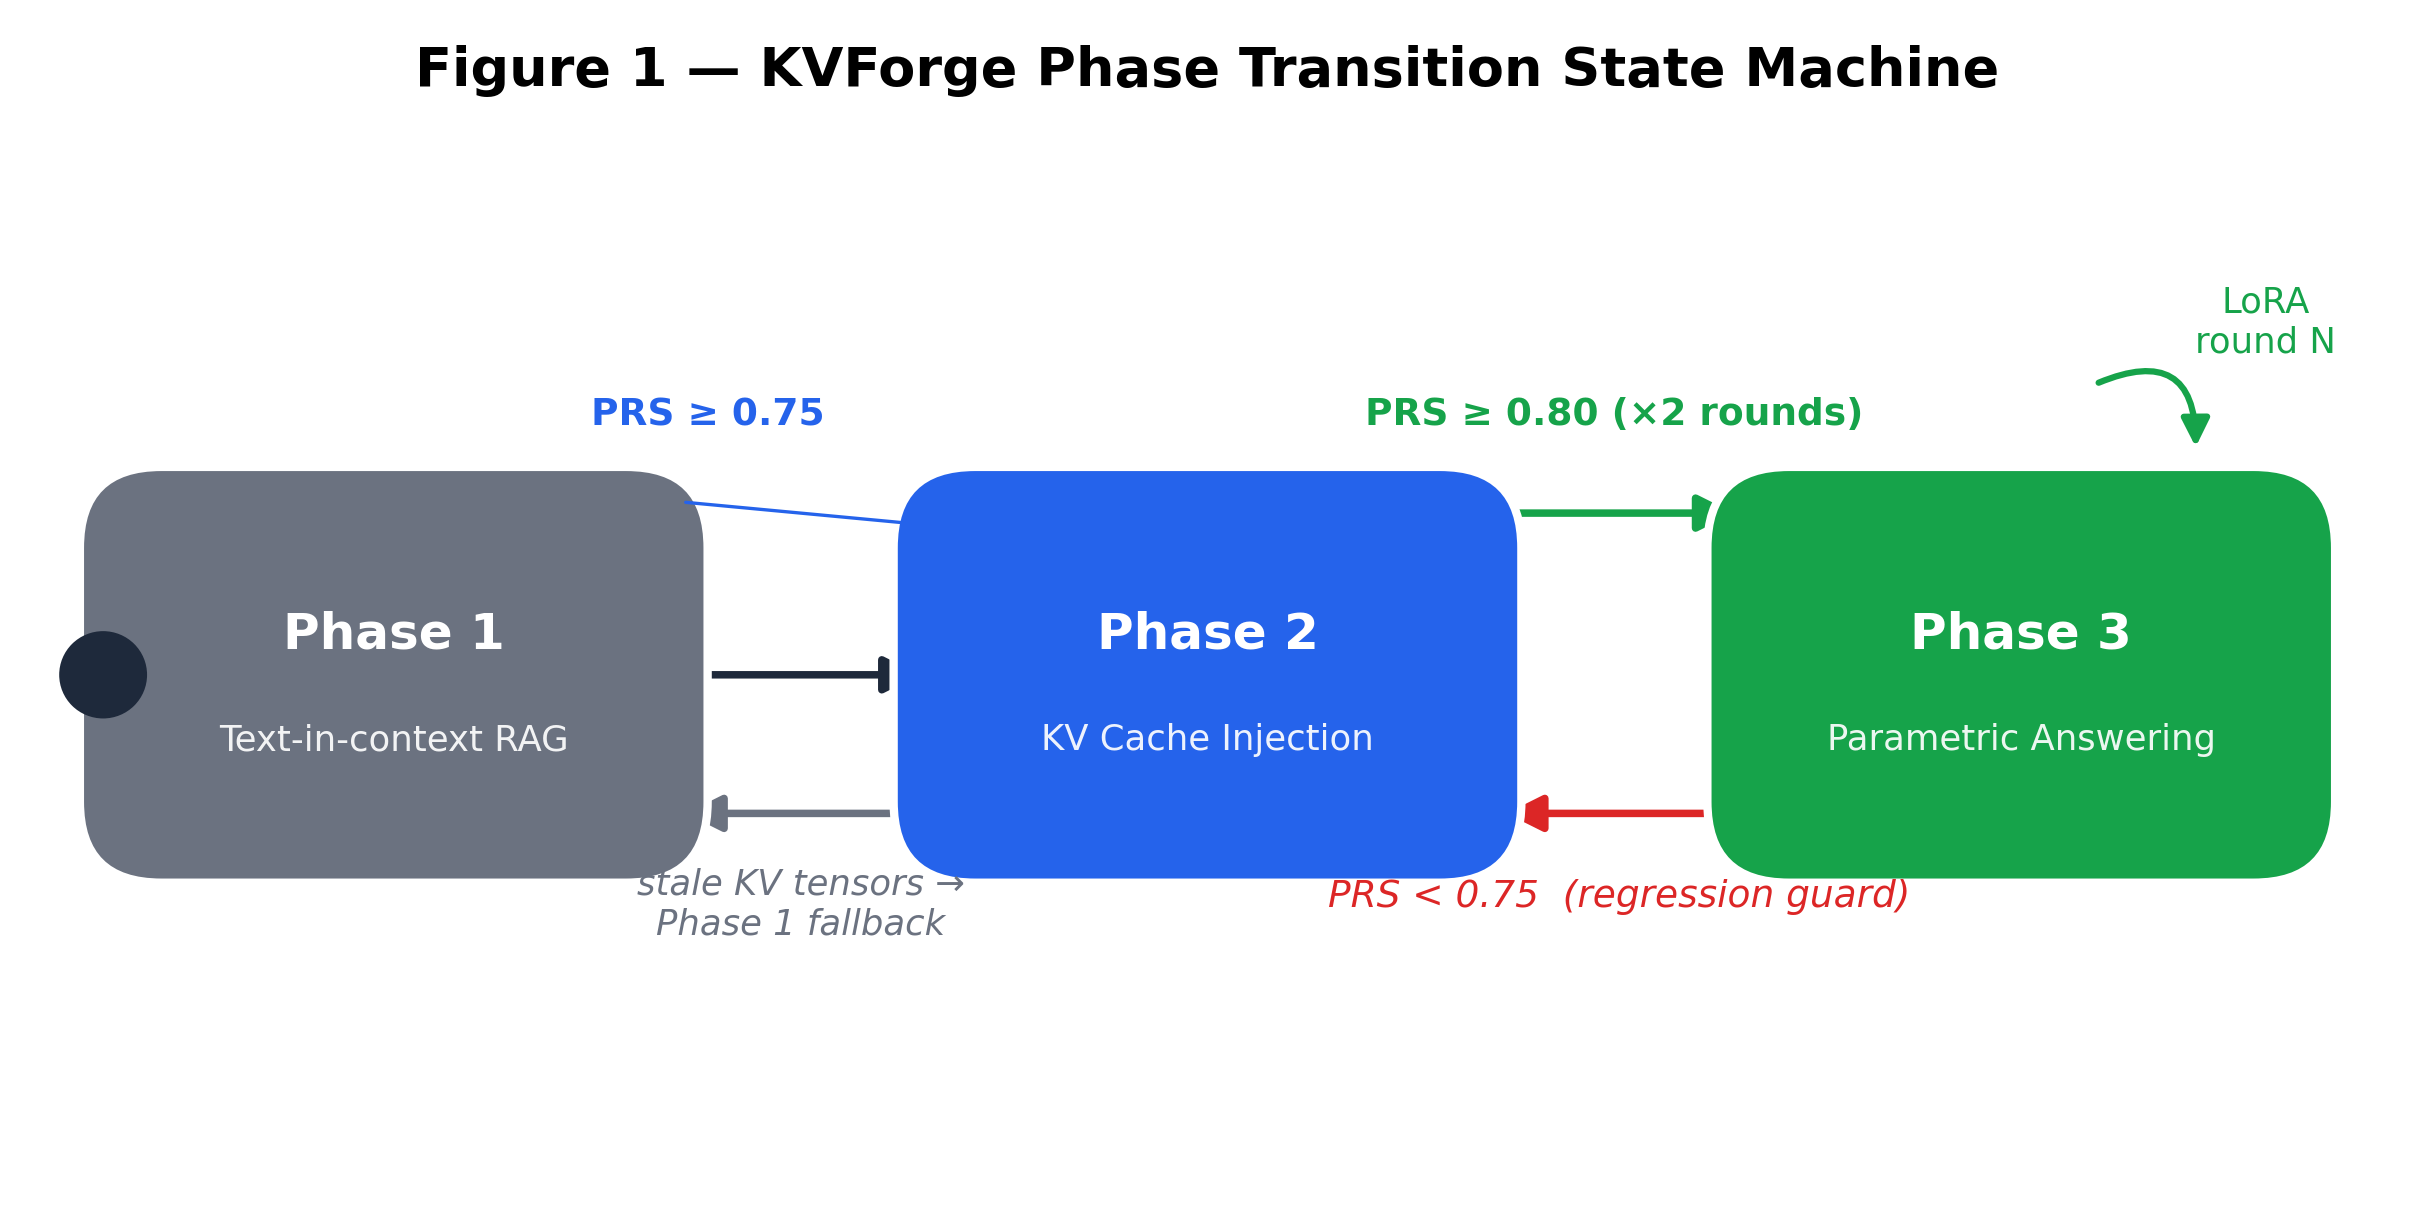
\includegraphics[width=\linewidth]{figures/fig01_phase_state_machine.png}
  \caption{Figure 1: KVForge Phase Transition State Machine}
  \label{fig:1}
\end{figure*}


Beyond the three phases, KVForge introduces two systems addressing storage and curation challenges at scale:


\textbf{Corpus Importance Score (CIS)} is a multi-signal chunk importance metric combining log-normalized retrieval frequency, semantic uniqueness ($1 -$ max cosine similarity to any neighbor), and FAQ topic coverage.


\textbf{TurboQuant} \cite{ref38} (Google DeepMind, 2025) compresses the full per-token KV sequence to 3 bits per key coordinate and 4 bits per value coordinate, achieving 4.4$\times$ compression over float16 while preserving attention-score quality for direct computation without decompression. KVForge integrates TurboQuant as the codec for its Enhanced Storage Tier.


This paper makes the following contributions:


\begin{enumerate}
  \item \textbf{KVForge architecture}: a unified system combining vector database retrieval, durable KV tensor storage, access-tier tracking, sleep-time FAQ generation, LoRA fine-tuning, and PRS-gated phase transitions.
  \item \textbf{Parametric Readiness Score (PRS)}: a principled composite metric for evaluating parametric knowledge retention and gating autonomous phase advancement.
  \item \textbf{Corpus Importance Score (CIS)}: a multi-signal importance metric for chunk-level storage curation and resource allocation.
  \item \textbf{Integration of TurboQuant} \cite{ref38}: KVForge adopts the TurboQuant codec (Google DeepMind, 2025) for the Enhanced Storage Tier, demonstrating that a 4.4$\times$ compressed per-token KV representation enables full-token injection at tractable storage cost (\textasciitilde{}15 MB/chunk for 8B models).
  \item \textbf{Empirical evaluation} across four heterogeneous corpora demonstrating all four reach Phase 3 with PRS 0.755--0.863, with training signal quality as the dominant variable.
\end{enumerate}



\section{Background}

\subsection{Transformer Attention and the KV Cache}

The scaled dot-product attention mechanism \cite{ref2} for query matrix \textbf{Q}, key matrix \textbf{K}, and value matrix \textbf{V} is:


\[
  \mathrm{Attention}(Q, K, V) = \mathrm{softmax}(Q K^\top / \sqrt{d_{k}}) \cdot V
\]

During autoregressive generation, the model maintains a \textit{KV cache}: after processing the input prompt, the \textbf{K} and \textbf{V} projections for every input token are saved so they need not be recomputed during subsequent generation steps. For a single decoder layer with \textit{n\_h} KV heads of dimension \textit{d\_h}, the KV cache for a sequence of length \textit{L} occupies:


\[
  size = 2 \times  L \times  n_{h} \times  d_{h} \times  sizeof(dtype)  bytes
\]

Standard RAG builds a fresh KV cache from scratch for each query. KVForge pre-builds it for every document chunk at index time and stores it persistently.


\subsection{Low-Rank Adaptation (LoRA)}

LoRA \cite{ref4} adapts a frozen pre-trained weight matrix \textbf{W$_0$ $\in$ $\mathbb{R}$\textasciicircum{}(d$\times$k)} via a low-rank decomposition:


\begin{lstlisting}
W = W0 + dW = W0 + BA
\end{lstlisting}

where \textbf{B $\in$ $\mathbb{R}$\textasciicircum{}(d$\times$r)} and \textbf{A $\in$ $\mathbb{R}$\textasciicircum{}(r$\times$k)}, with rank r $\ll$ min(d, k). KVForge applies LoRA to \texttt{q\_proj}, \texttt{k\_proj}, and \texttt{v\_proj} attention matrices. Because LoRA updates the \textbf{K} and \textbf{V} projections, any stored KV tensors become stale after a LoRA round and must be recomputed --- tracked per-chunk via a \texttt{kv\_version} field.


\subsection{KV Cache Quantization}

Keys and values have different statistical properties: keys have high inter-channel variance benefiting from column-wise quantization, while values have smoother distributions amenable to group quantization \cite{ref30,ref31}. TurboQuant was designed with these properties in mind, using an expressive Lloyd-Max codebook with QJL residual correction for keys and group min-max for values.


\subsection{Retrieval-Augmented Generation}

Lewis et al. \cite{ref1} introduced RAG combining a non-parametric retrieval index with a parametric pre-trained generator. KVForge's distinct position: rather than improving retrieval, it progressively \textit{eliminates} retrieval for queries the model has memorized, while preserving retrieval as a fallback.



\section{Related Work}

\subsection{KV Cache Reuse and Prefix Caching}

\textbf{PromptCache} \cite{ref8} modularizes the KV cache for reuse across queries sharing a common prompt prefix. KVForge operates at a different layer: where PromptCache operates within a single inference server session and loses its cache on restart, KVForge persists KV tensors durably in a vector database across server restarts, model updates, and distributed replicas.


\textbf{PagedAttention} \cite{ref3} and \textbf{vLLM} manage KV memory within a single server process using virtual memory paging. KVForge operates at the pre-retrieval layer --- deciding \textit{which} chunks' KV tensors to supply --- while vLLM manages how they are stored during generation. The systems are complementary.


\textbf{SGLang} \cite{ref9} provides a radix-tree prefix cache achieving >99\% prefix reuse on shared prompts. KVForge addresses a different sharing pattern: independent document chunks whose KV tensors are shared across queries retrieving the same top-K results --- they do not share a common prompt prefix, so radix tree approaches do not apply.


\textbf{CacheBlend} \cite{ref32} reuses KV caches of retrieved segments by selectively recomputing tokens whose attention deviates substantially from the pre-computed cache. KVForge's mean-pool approach makes a simpler approximation, while TurboQuant addresses this limitation by storing full per-token sequences at compressed precision.


\subsection{RAG Systems and Dense Retrieval}

\textbf{DPR} \cite{ref5} demonstrated that jointly-trained dual encoders outperform BM25 for open-domain QA. \textbf{ColBERT} \cite{ref29} introduced late interaction with per-token embeddings. \textbf{RETRO} \cite{ref10} pre-computes chunk encodings at index time and conditions generation on retrieved neighbours. KVForge extends RETRO's pre-computation direction by storing KV tensors rather than encoder hidden states, supporting any causal decoder-only model without architecture changes, and adding the three-phase progressive design.


\textbf{FiD} \cite{ref33} encodes multiple retrieved passages independently and fuses them in the decoder. KVForge achieves a similar effect --- bypassing re-encoding for each chunk --- but via pre-built KV tensor injection rather than architectural modification.


\subsection{LoRA and Parameter-Efficient Fine-Tuning}

\textbf{QLoRA} \cite{ref12} enables 4-bit quantized LoRA training, reducing GPU memory from \textasciitilde{}12 GB to \textasciitilde{}4 GB for a 7B model. KVForge supports QLoRA via \texttt{bitsandbytes} NF4 quantization.


\textbf{Continual LoRA fine-tuning} risks catastrophic forgetting \cite{ref18}. KVForge's \textbf{tier-weighted replay buffer} mitigates this: hot chunks receive 8$\times$ sampling weight relative to frozen chunks, acting as a lightweight proxy for Elastic Weight Consolidation \cite{ref34}.


\subsection{Calibration and Uncertainty Estimation}

\textbf{Guo et al.} \cite{ref13} proposed temperature scaling for calibration. KVForge's PRS calibration component uses a self-reporting proxy (model rates its own confidence 0--100) aligned with semantic accuracy. \textbf{Self-Consistency} \cite{ref14} samples multiple reasoning chains for agreement. KVForge's consistency component computes mean pairwise cosine similarity across three sampled answers at temperature 0.7. \textbf{Semantic Entropy} \cite{ref16} provides model-agnostic uncertainty estimates; KVForge's Phase 3 gate uses a lighter three-signal combination to avoid multi-sample generation overhead.


\subsection{KV Cache Compression}

\textbf{KVQuant} \cite{ref30} quantizes KV caches to 1--4 bits using non-uniform per-channel quantization. \textbf{KIVI} \cite{ref31} applies asymmetric 2-bit quantization achieving 2.2$\times$ compression. \textbf{QJL} \cite{ref35} proposes a quantized Johnson-Lindenstrauss transform for unbiased inner-product estimation from sign bits. \textbf{TurboQuant} \cite{ref38} (Google DeepMind, 2025) synthesizes all three: QJL rotation preprocessing, Lloyd-Max scalar quantization for MSB representation, and QJL sign bits for residual correction. KVForge adopts TurboQuant as the codec for its Enhanced Storage Tier.


\subsection{Continual Learning}

\textbf{Online Continual Learning} surveys \cite{ref37} identify replay-based methods as most practical for production systems. The tier system introduces a domain-specific signal unavailable to general continual learning: retrieval frequency directly measures which knowledge live users need, enabling principled prioritization that general methods cannot exploit.



\section{The KVForge System}

\subsection{Architecture Overview}

\textbf{Figure 2} shows the full KVForge system architecture. The system operates as a state machine with an offline pipeline (left path) and an online query path (right path), connected by the access tracking and tier classification loop.


\begin{figure*}[htbp]
  \centering
  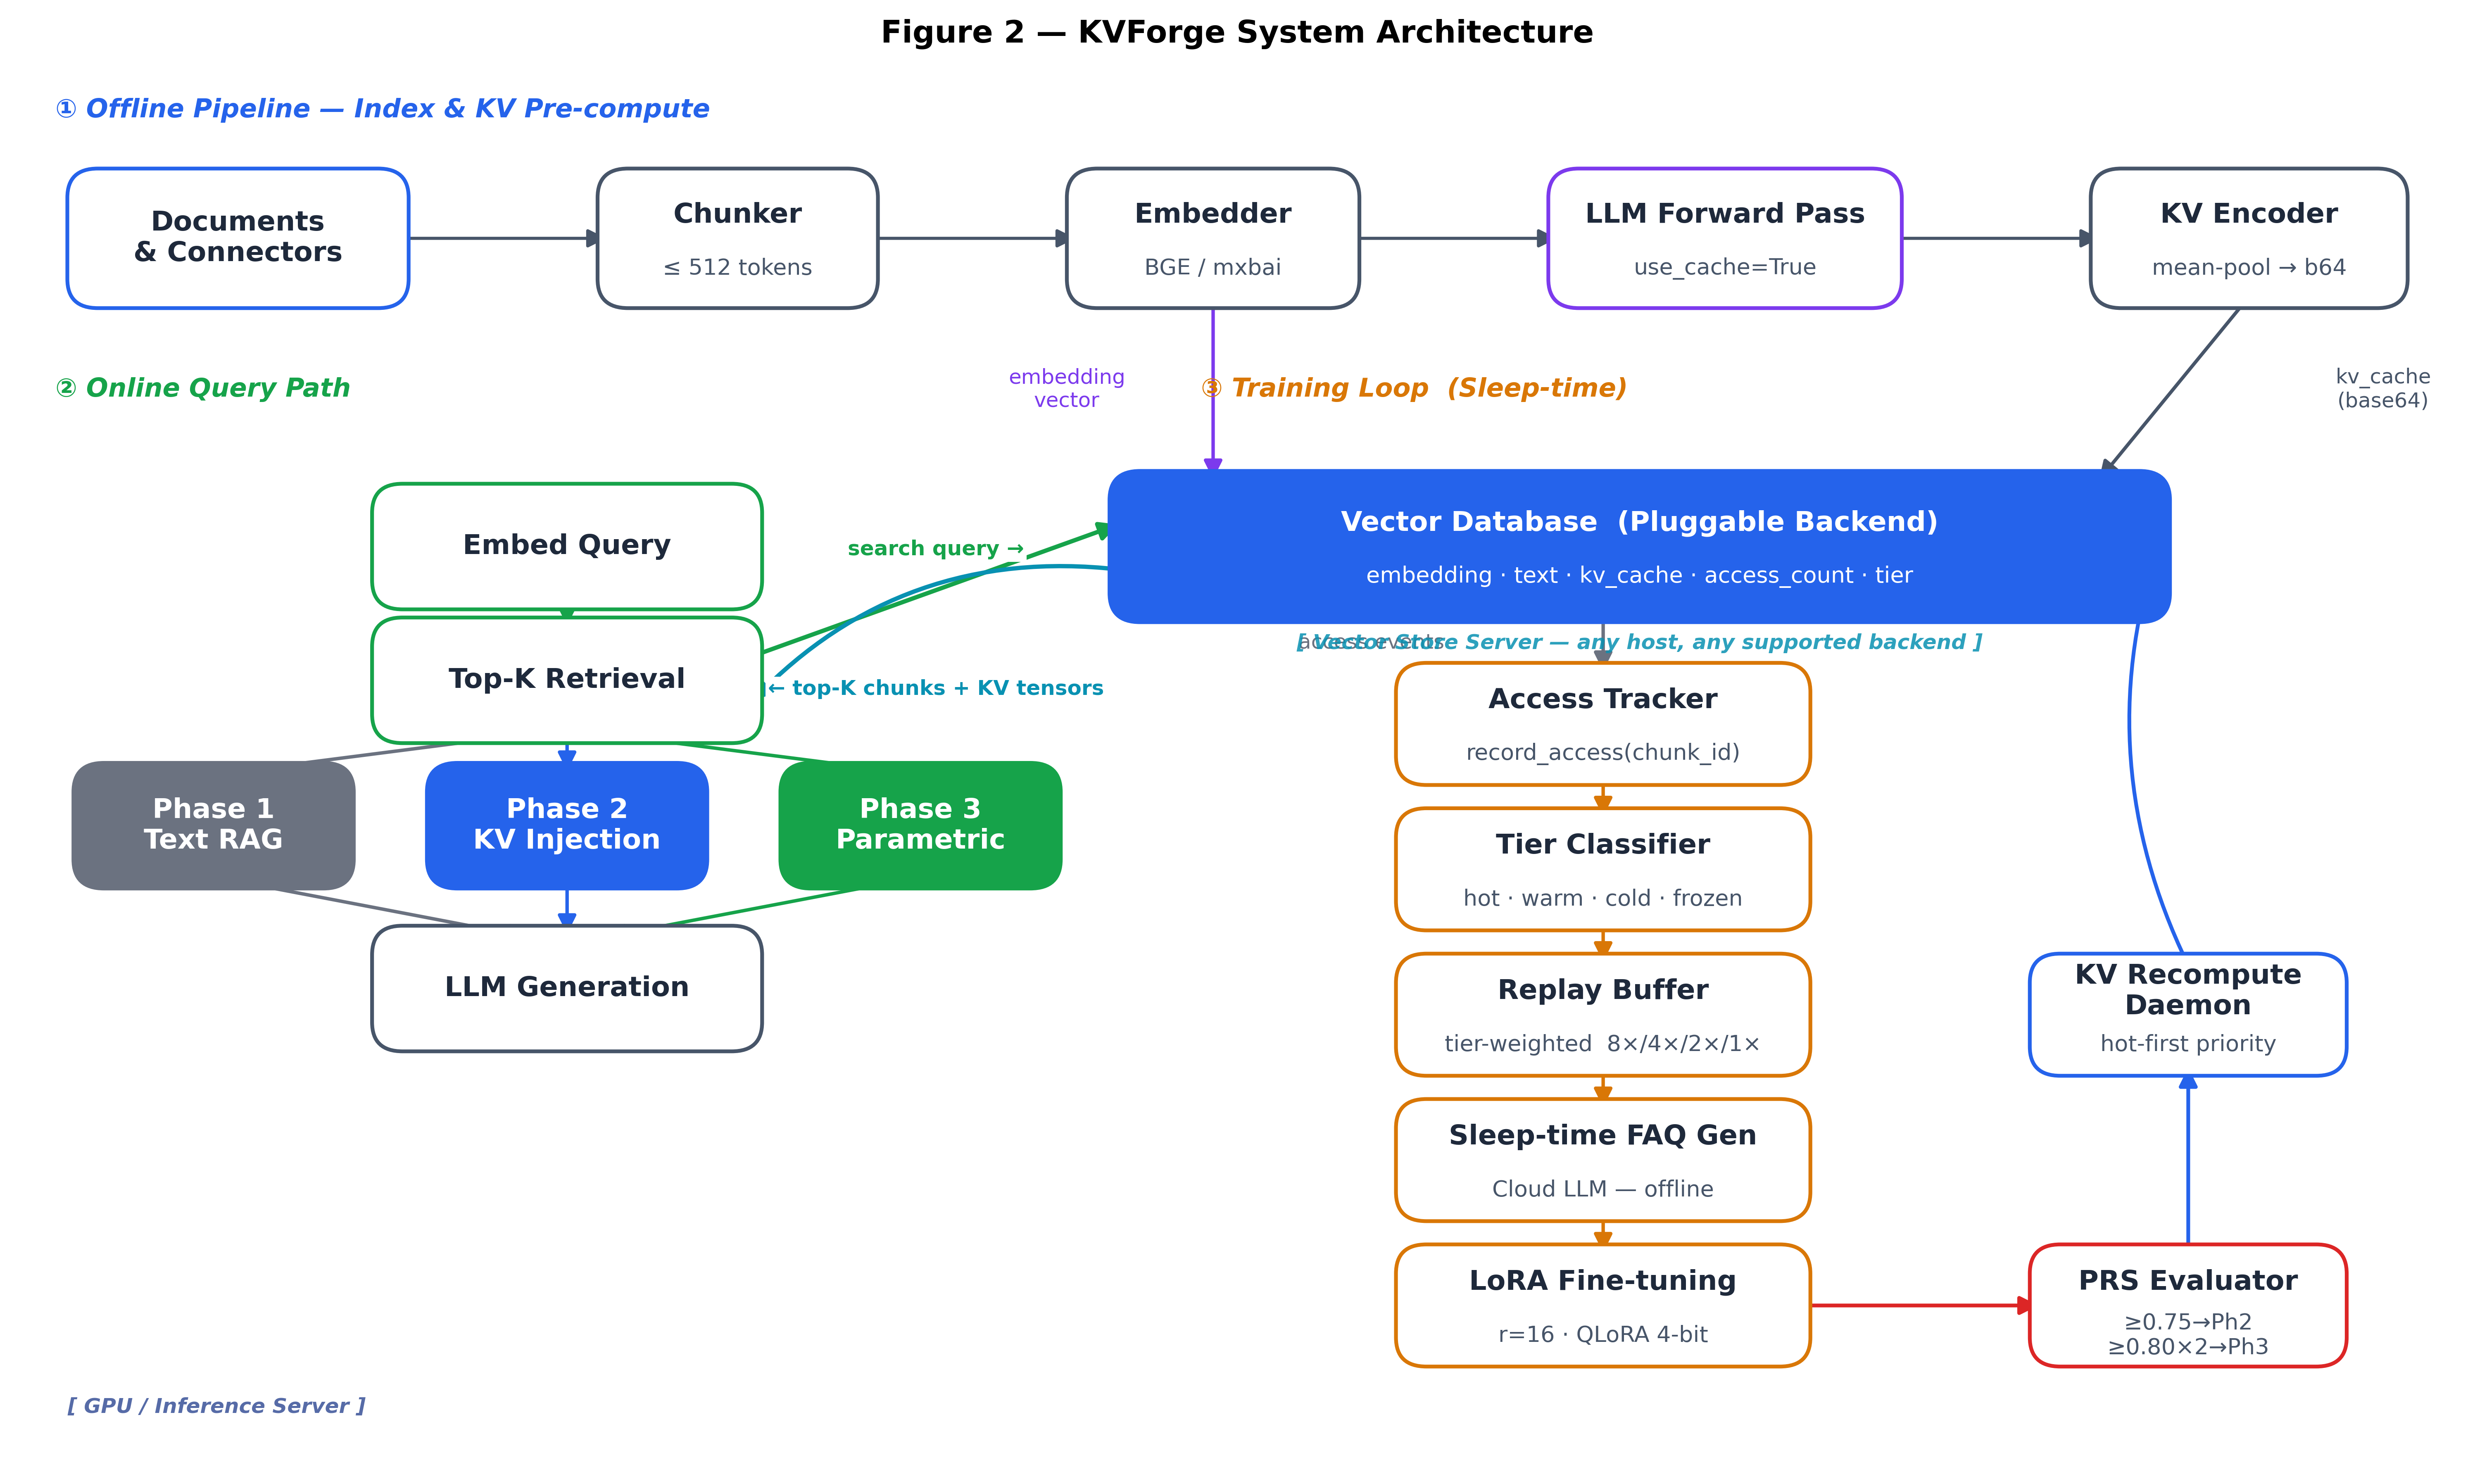
\includegraphics[width=\linewidth]{figures/fig02_system_architecture.png}
  \caption{Figure 2: Full KVForge system architecture. Offline pipeline pre-computes KV tensors and trains the LoRA adapter. Online query path injects pre-built KV tensors. Access tracking closes the loop from live traffic to training.}
  \label{fig:2}
\end{figure*}


The overall pipeline sequence is:


\begin{lstlisting}
Index -> KV Pre-compute -> [Phase 1]
     -> Sleep-time FAQ Gen -> LoRA Train -> KV Recompute -> PRS Eval -> [Phase 2]
     -> LoRA Train (round 2) -> KV Recompute -> PRS Eval -> [Phase 3]
        ^____________________continuous improvement loop________________________^
\end{lstlisting}

System state is stored atomically in a \texttt{version.json} file per corpus, updated via temp-file rename to prevent corruption:


\begin{lstlisting}
{
  "current_lora_version": 4,
  "checkpoint_path": "lora_checkpoints/v4/",
  "phase": 3,
  "prs_history": [
    {"round": 1, "prs": 0.727},
    {"round": 2, "prs": 0.783},
    {"round": 3, "prs": 0.863}
  ],
  "known_good_queries": [...]
}
\end{lstlisting}

\subsection{Indexing and KV Pre-computation}

At index time each document chunk undergoes a two-stage process:


\textbf{Stage 1 --- Embedding and upsert.} The chunk text is embedded by the configured encoder (default: BAAI/bge-small-en-v1.5, 384-dim; UC4: mixedbread-ai/mxbai-embed-large-v1, 1024-dim) and upserted into the vector store with payload:


\begin{lstlisting}
{
  "text": "...", "page": 3, "source_file": "guide.pdf",
  "access_count": 0, "kv_version": null, "tier": "frozen"
}
\end{lstlisting}

\textbf{Stage 2 --- KV tensor computation.} The chunk is tokenized (truncated to 512 tokens) and passed through the LLM:


\begin{lstlisting}
outputs = model(**inputs, use_cache=True)
kv = outputs.past_key_values   # tuple of (K, V) per layer
\end{lstlisting}

Per-layer tensors \texttt{[1, n\_kv\_heads, seq\_len, head\_dim]} are mean-pooled over the sequence dimension, stacked into shape \texttt{[L, 2, H, d\_h]}, serialized to float16, and stored as base64 in the Qdrant payload field \texttt{kv\_cache}.


For Llama-3.2-3B-Instruct (28 layers, 8 KV heads, head\_dim=128):


\begin{lstlisting}
28 * 2 * 8 * 128 * 2 bytes ~ 57 KB per chunk
2,520 chunks * 57 KB ~ 143 MB total (UC4)
\end{lstlisting}

\subsection{Query-Time Inference: Phase 1 vs Phase 2}

\textbf{Figure 3} contrasts the two retrieval-based inference paths.


\begin{figure*}[htbp]
  \centering
  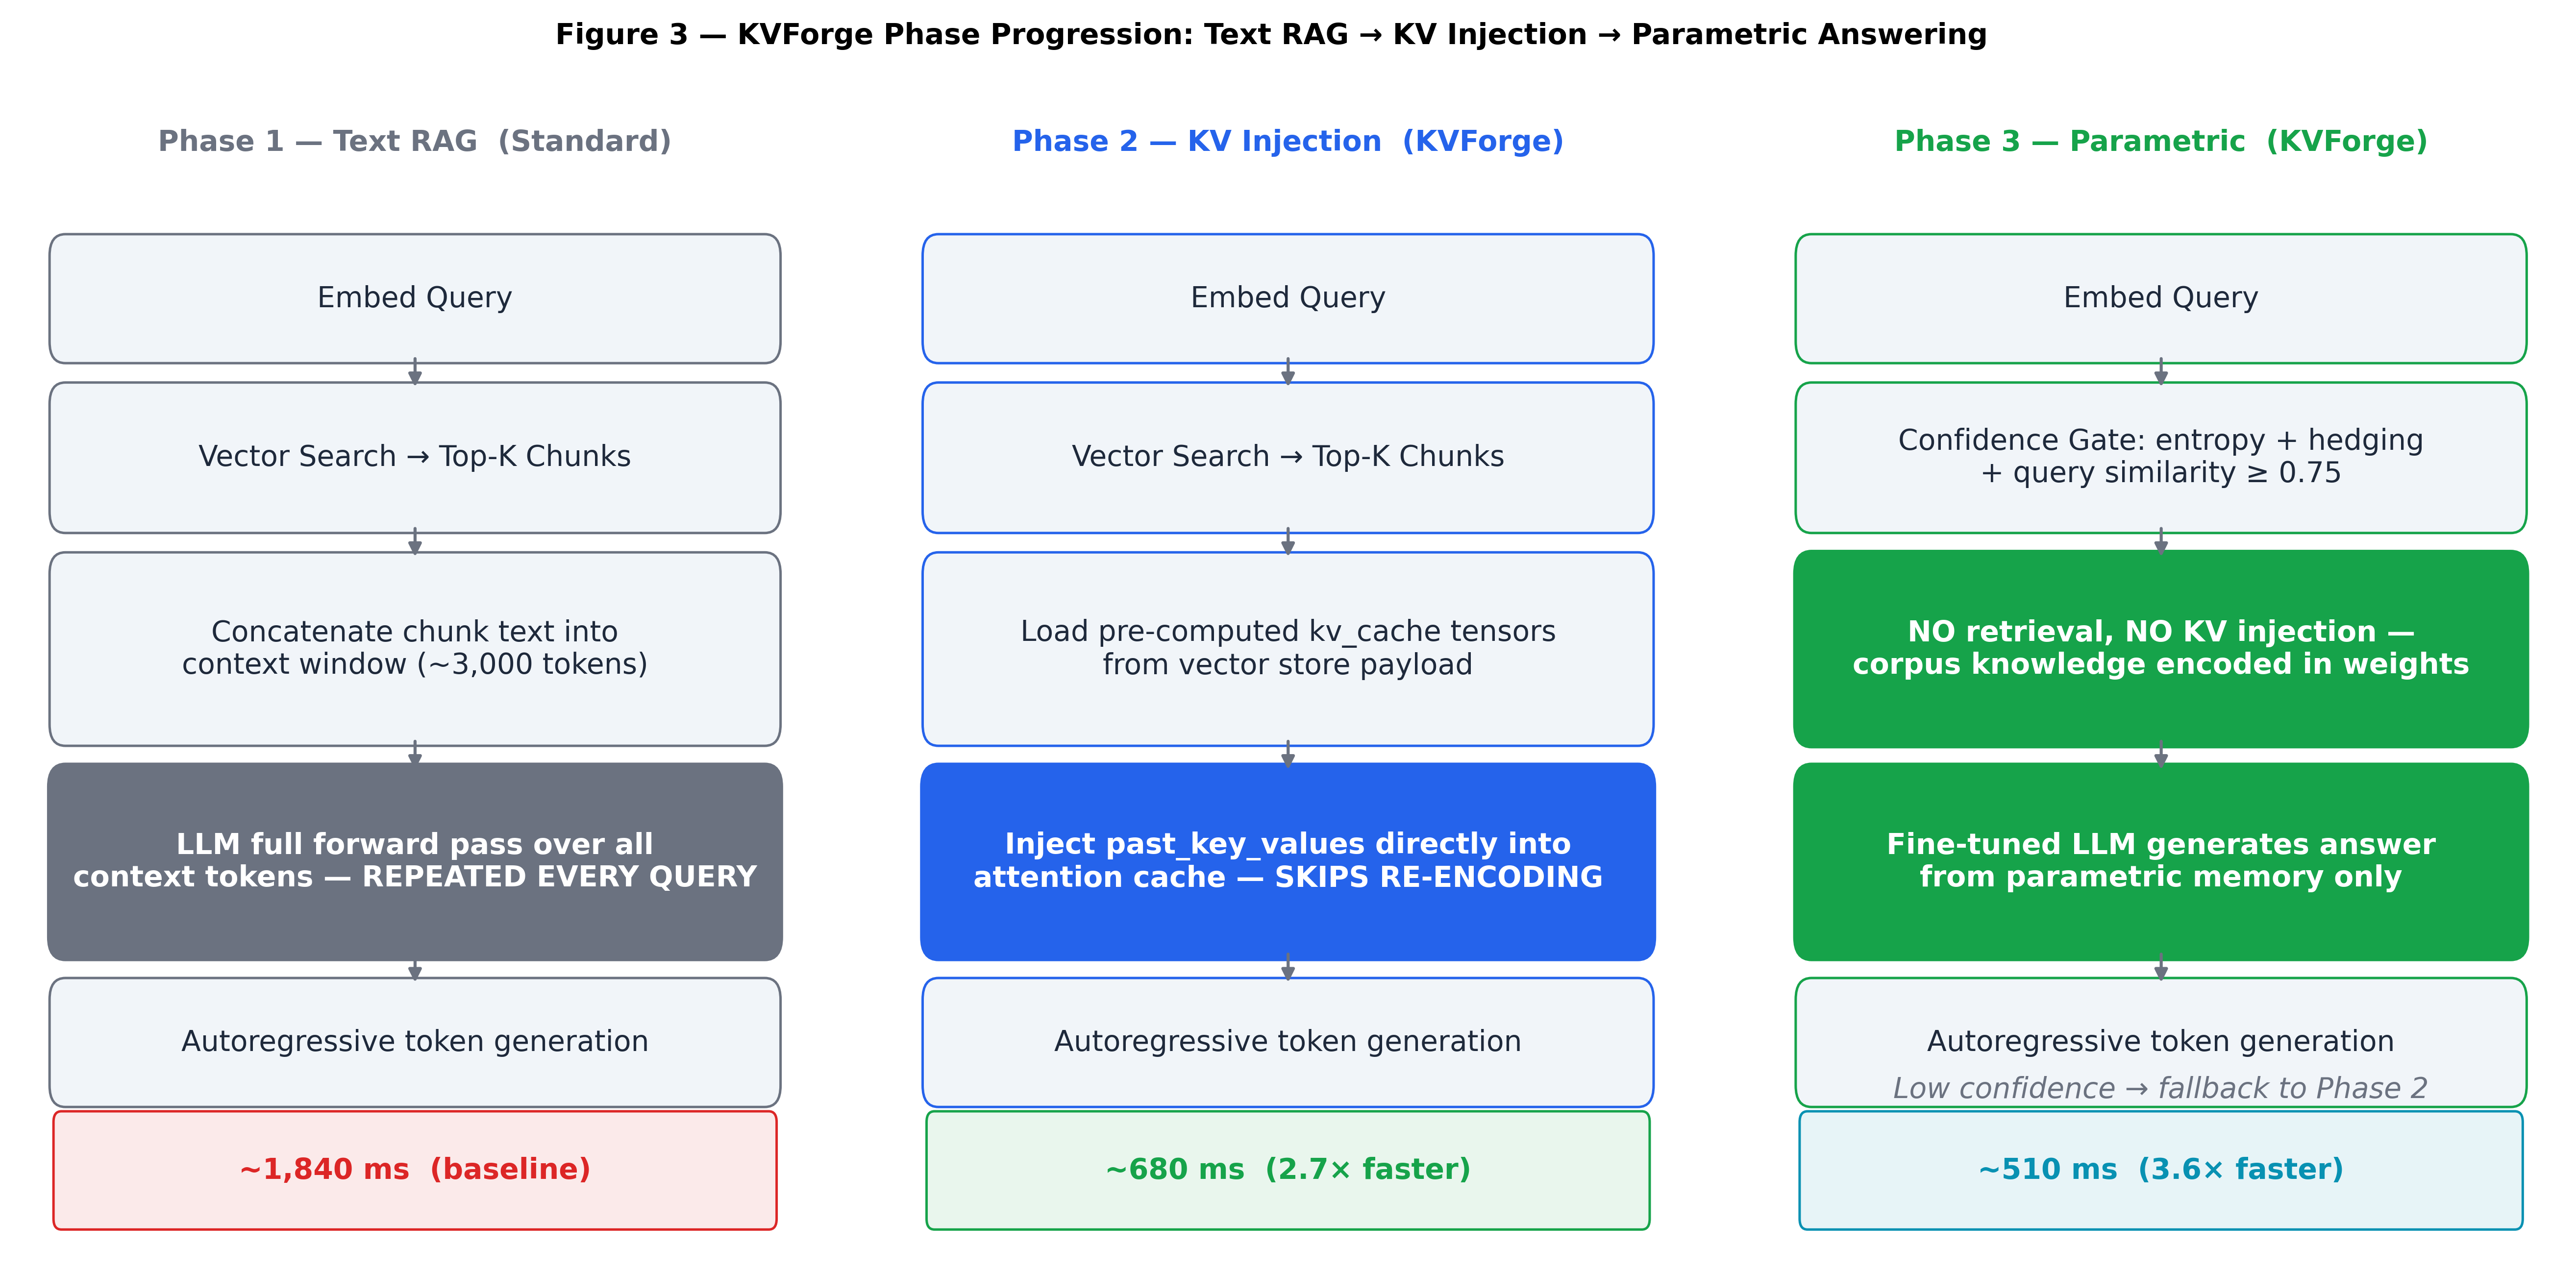
\includegraphics[width=\linewidth]{figures/fig03_rag_vs_kv_injection.png}
  \caption{Figure 3: Standard Text RAG vs KV Cache Injection. Phase 1 performs a full LLM forward pass over retrieved text on every query (\textasciitilde{}1,840 ms). Phase 2 injects pre-computed KV tensors directly, skipping re-encoding (\textasciitilde{}680 ms, 2.7$\times$ speedup).}
  \label{fig:3}
\end{figure*}


At query time, the inference module: (1) embeds the query and retrieves top-K chunks; (2) compares each chunk's \texttt{kv\_version} against \texttt{current\_lora\_version}; (3) if \textbf{all} chunks are fresh, injects their KV tensors via \texttt{past\_key\_values}; (4) if \textbf{any} chunk is stale, falls back to Phase 1 text-in-context for the entire query and enqueues stale chunks for background recomputation.


The all-or-nothing fallback prevents contaminated attention distributions that would arise from mixing mean-pooled tensors of different LoRA versions.


\subsection{Sleep-Time FAQ Generation}

Before each LoRA training round, the \texttt{sleep\_faq\_generator} queries a cloud LLM (Gemini 2.5 Flash, Claude, or GPT-4.1) to generate N diverse question-answer pairs per chunk. This is sleep-time compute \cite{ref19}: offline work that improves future inference quality without impacting query latency.


\textbf{Prompt template (per chunk):}


\begin{lstlisting}
Given the following document passage, generate {count} diverse, specific
question-answer pairs that a real user might ask. Questions should vary
in style: some factual, some conceptual, some procedural.

Passage: {chunk_text}

Return as JSON array: [{"question": "...", "answer": "..."}, ...]
\end{lstlisting}

With tier weighting active, the question budget is allocated proportional to tier weight. For a 50-question budget across 2,520 chunks, \textasciitilde{}50\% of questions target the top-15\% hot chunks, concentrating training signal on knowledge that matters to live user traffic.


\subsection{Tier-Weighted Replay Buffer}

\textbf{Figure 4} shows the tier weight system. The SQLite replay buffer (\texttt{core/replay\_buffer.py}) stores \texttt{(chunk\_id, text, tier)} rows derived from generated FAQs. Table~\ref{tab:replay-buffer} lists the tier conditions and replay weights.


\begin{figure*}[t]
  \centering
  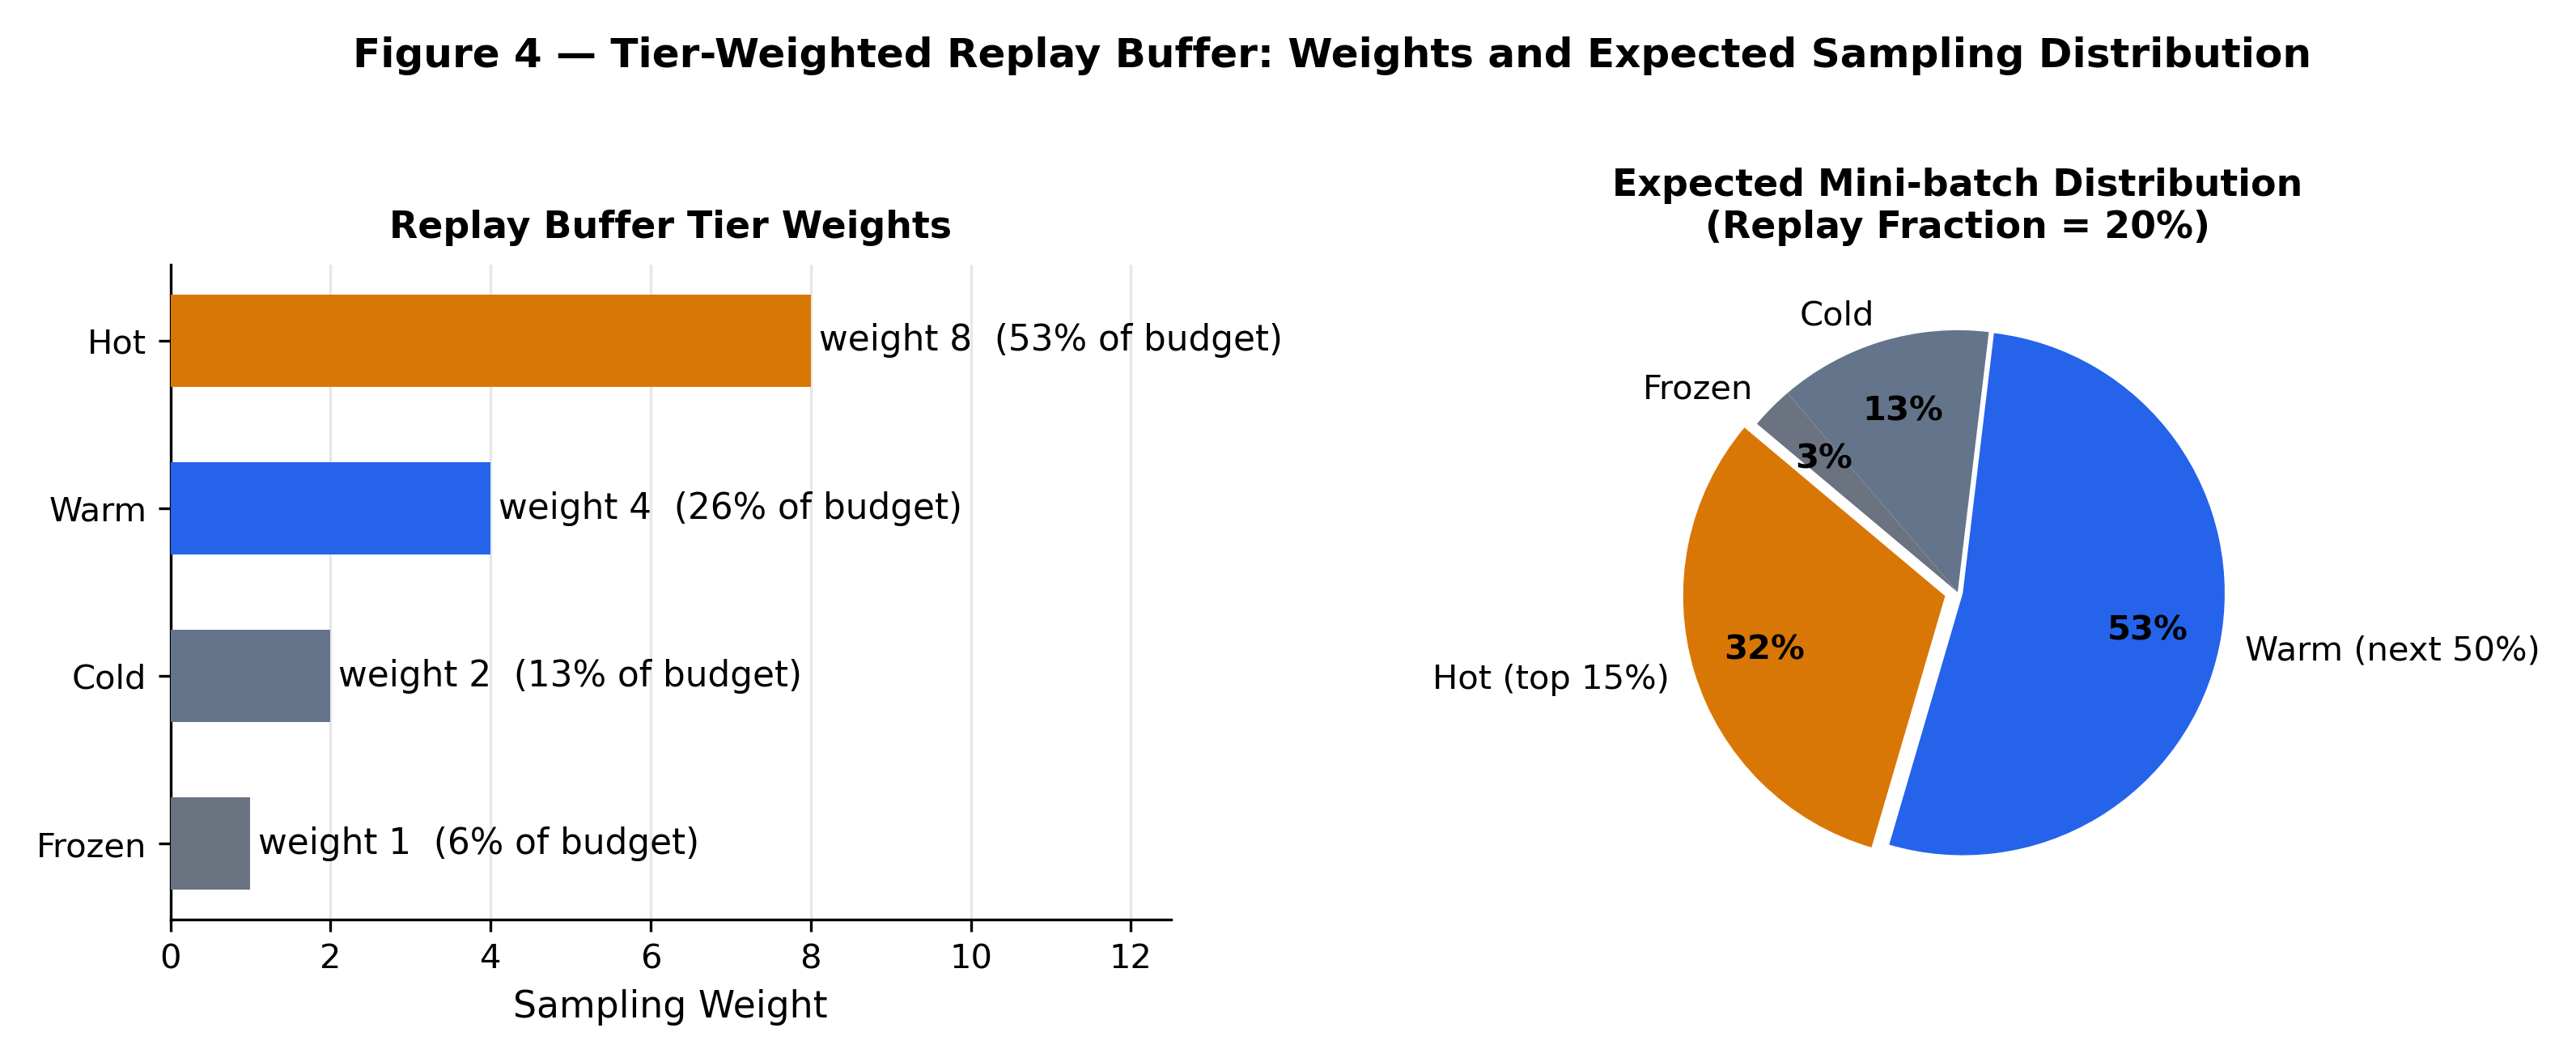
\includegraphics[width=\linewidth]{figures/fig04_tier_weights.png}
  \caption{Figure 4: Tier-Weighted Replay Buffer. Hot chunks (top 15\% by access count, accessed within 7 days) receive 8$\times$ replay weight. The pie chart shows the expected mini-batch distribution when the replay fraction is 20\%.}
  \label{fig:4}
\end{figure*}


\begin{table*}[htbp]
  \centering\small
  \caption{Tier-Weighted Replay Buffer: access tier conditions and replay weights}
  \label{tab:replay-buffer}
  \begin{tabularx}{\textwidth}{lLl}
  \toprule
    Tier & Condition & Replay weight \\
  \midrule
  \midrule
  hot & Top 15\% by access count, last accessed < 7 days & 8 \\
  warm & Next 50\%, last accessed < 30 days & 4 \\
  cold & Remaining accessed chunks & 2 \\
  frozen & Never accessed & 1 \\
  \bottomrule
  \end{tabularx}
\end{table*}


The buffer evicts the lowest-tier and oldest entries when exceeding a capacity cap (default: 5,000 chunks), bounding memory regardless of corpus growth.


\subsection{LoRA Fine-Tuning Loop}

HuggingFace PEFT LoRA fine-tuning configuration:


\begin{itemize}
  \item \textbf{Targets:} \texttt{q\_proj}, \texttt{k\_proj}, \texttt{v\_proj} attention projections
  \item \textbf{Rank:} r = 16, alpha = 32 (effective scaling $\alpha$/r = 2)
  \item \textbf{Quantization:} 4-bit NF4 (QLoRA \cite{ref12}) via \texttt{bitsandbytes}
  \item \textbf{Replay fraction:} 20\% of each batch drawn from the replay buffer by tier weight
  \item \textbf{Epochs:} 3 per training round
\end{itemize}


After training, \texttt{kv\_version} is incremented and all stored KV tensors become stale, triggering the KV recompute phase. Hot chunks (top 15\%, \textasciitilde{}378 chunks for UC4) are recomputed first in \textasciitilde{}76 seconds, restoring Phase 2 quality for the majority of live queries before the full recompute completes.


\subsection{Parametric Readiness Score (PRS)}

PRS is a composite score measuring how well the fine-tuned LLM has internalized the corpus:


\[
  PRS = 0.5 \times  accuracy_{ratio} + 0.3 \times  calibration + 0.2 \times  consistency
\]

\textbf{Accuracy ratio} (50\%): For each FAQ, the model generates a \textit{parametric} answer (no retrieval) and a \textit{RAG} answer (with context). Let sim($\cdot$,$\cdot$) denote cosine similarity to the ground truth:


\[
  accuracy_{ratio} = \mathrm{min}( \mathrm{sim}(param_{ans}, gt) / (\mathrm{sim}(rag_{ans}, gt) + \varepsilon ), 1.0 )
\]

This measures parametric quality \textit{relative to the RAG baseline}, making the metric robust to corpus-specific difficulty.


\textbf{Calibration} (30\%): The model self-rates its confidence in its parametric answer (0--100 scale). Calibration measures whether expressed confidence tracks actual quality:


\begin{lstlisting}
calibration = 1.0 - |self_confidence_normalized - sim(param_ans, gt)|
\end{lstlisting}

\textbf{Consistency} (20\%): Three independent answers are sampled at temperature 0.7. Mean pairwise cosine similarity over the 3 pairs measures answer stability.


\textbf{Figure 5} shows the PRS component breakdown for UC4 (final training round):


\begin{figure*}[t]
  \centering
  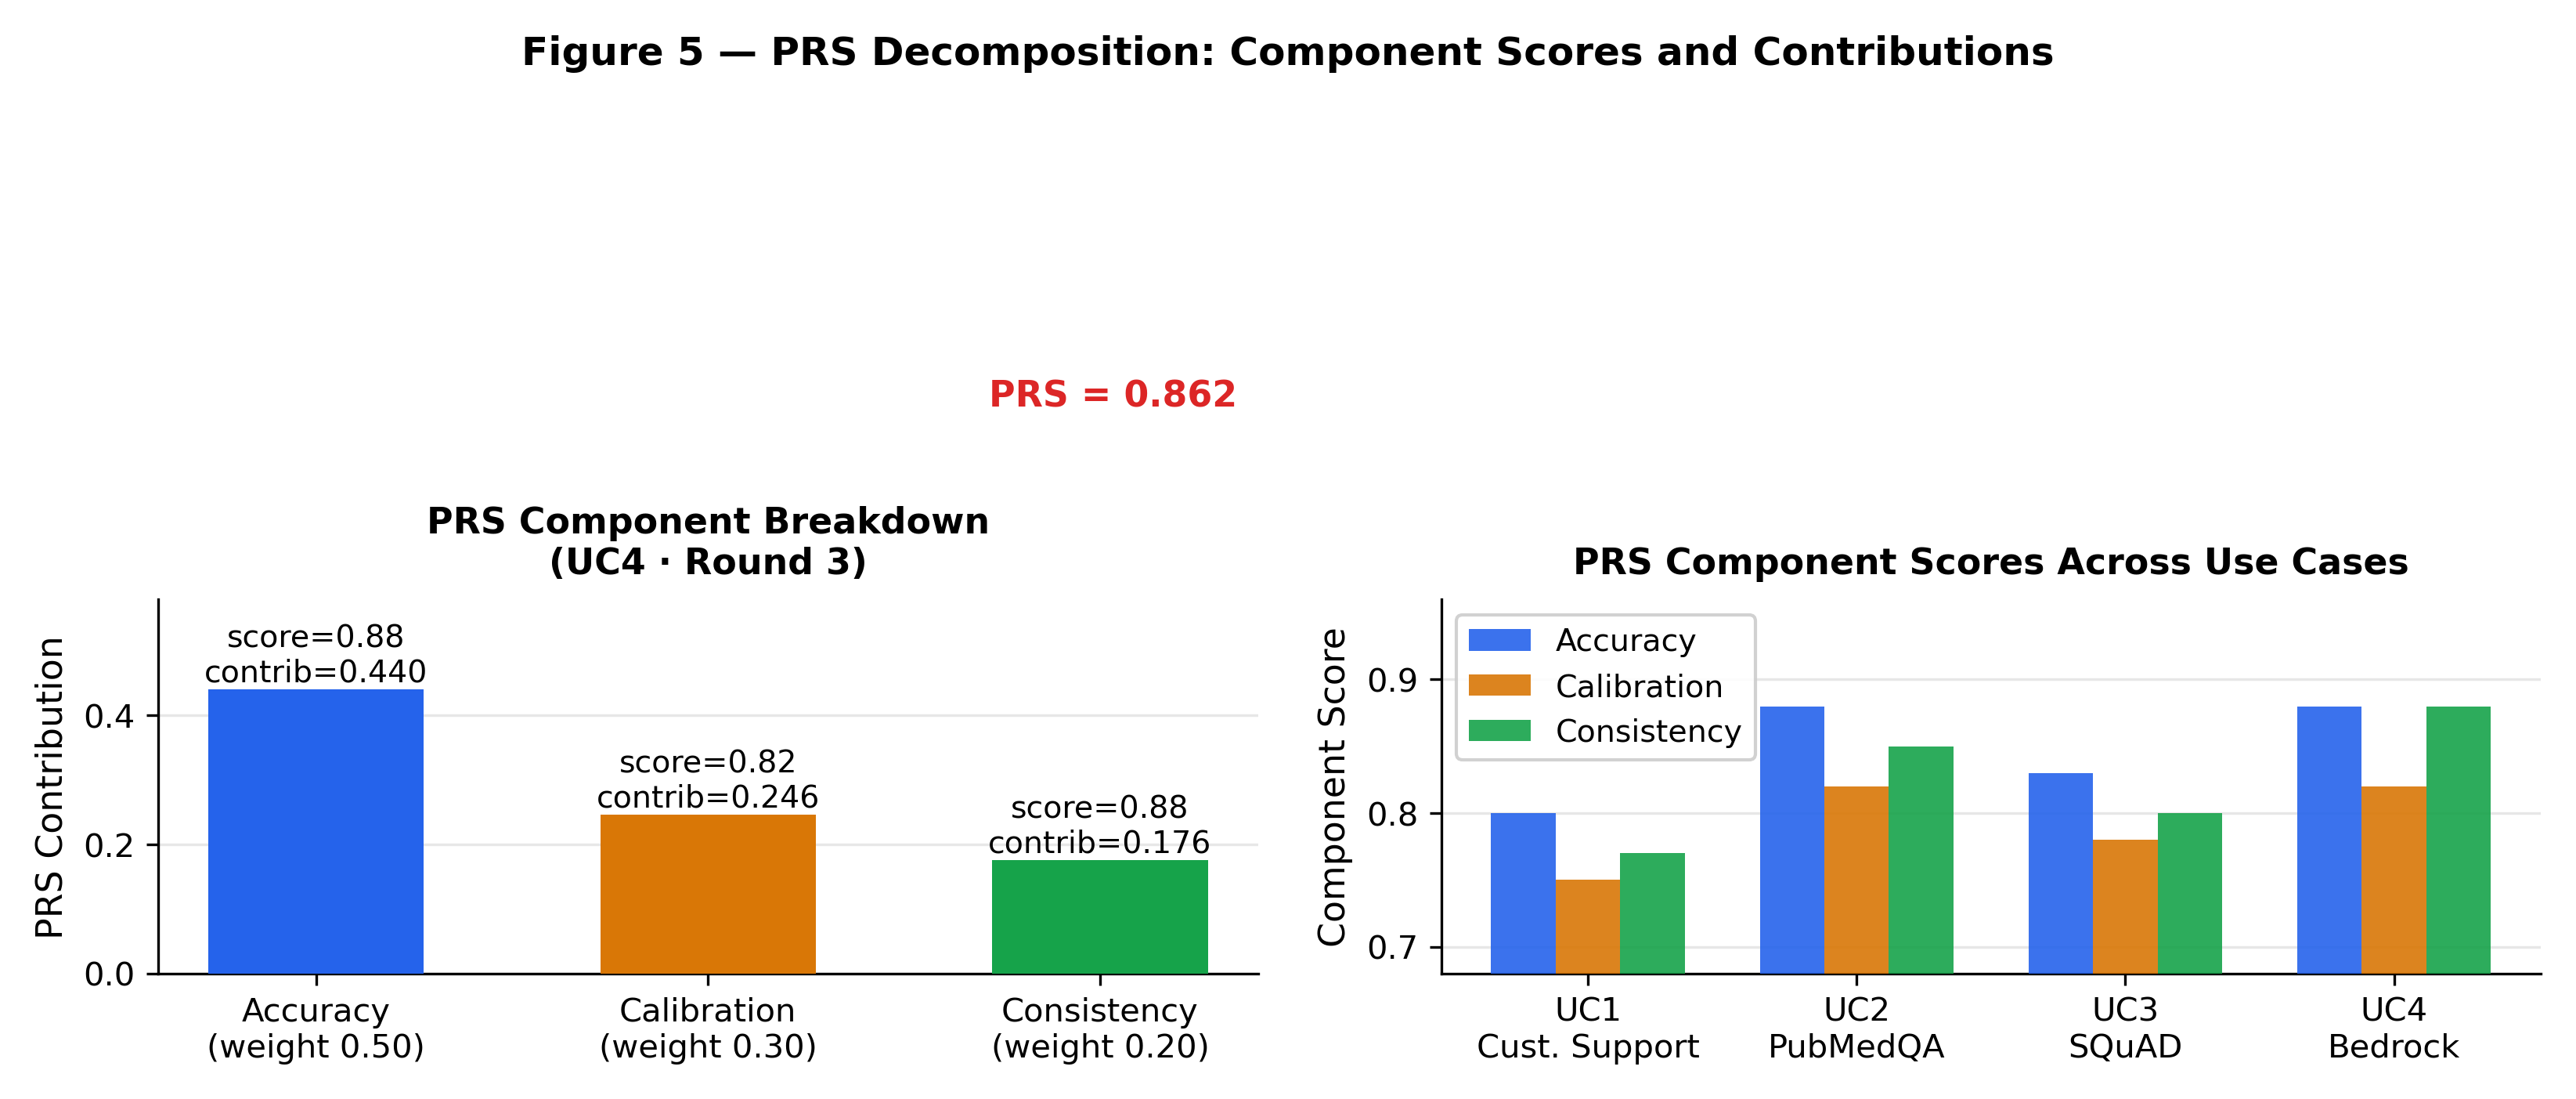
\includegraphics[width=\linewidth]{figures/fig05_prs_components.png}
  \caption{Figure 5: PRS Component Breakdown for UC4 (Amazon Bedrock User Guide, Round 3). Accuracy ratio 0.88 $\times$ 0.50 = 0.440; calibration 0.82 $\times$ 0.30 = 0.246; consistency 0.88 $\times$ 0.20 = 0.176; total PRS = 0.863.}
  \label{fig:5}
\end{figure*}


\textbf{Phase transition thresholds} (Table~\ref{tab:parametric-readiness-score-prs}):


\begin{table*}[htbp]
  \centering\small
  \caption{Parametric Readiness Score (PRS)}
  \label{tab:parametric-readiness-score-prs}
  \begin{tabularx}{\textwidth}{LL}
  \toprule
    Condition & Transition \\
  \midrule
  \midrule
  PRS $\geq$ 0.75, any single round & Phase 1 $\to$ Phase 2 \\
  PRS $\geq$ 0.80, two consecutive rounds & Phase 2 $\to$ Phase 3 \\
  PRS < 0.75 while in Phase 3 & Phase 3 $\to$ Phase 2 (regression guard) \\
  \bottomrule
  \end{tabularx}
\end{table*}


After each evaluation round, FAQ questions with \texttt{accuracy\_ratio} $\geq$ 0.85 are embedded and stored in \texttt{known\_good\_queries} in \texttt{version.json}, seeding the Phase 3 confidence gate.


\subsection{Phase 3 Confidence Gate}

\textbf{Figure 6} shows the decision logic for Phase 3 inference routing.


\begin{figure*}[t]
  \centering
  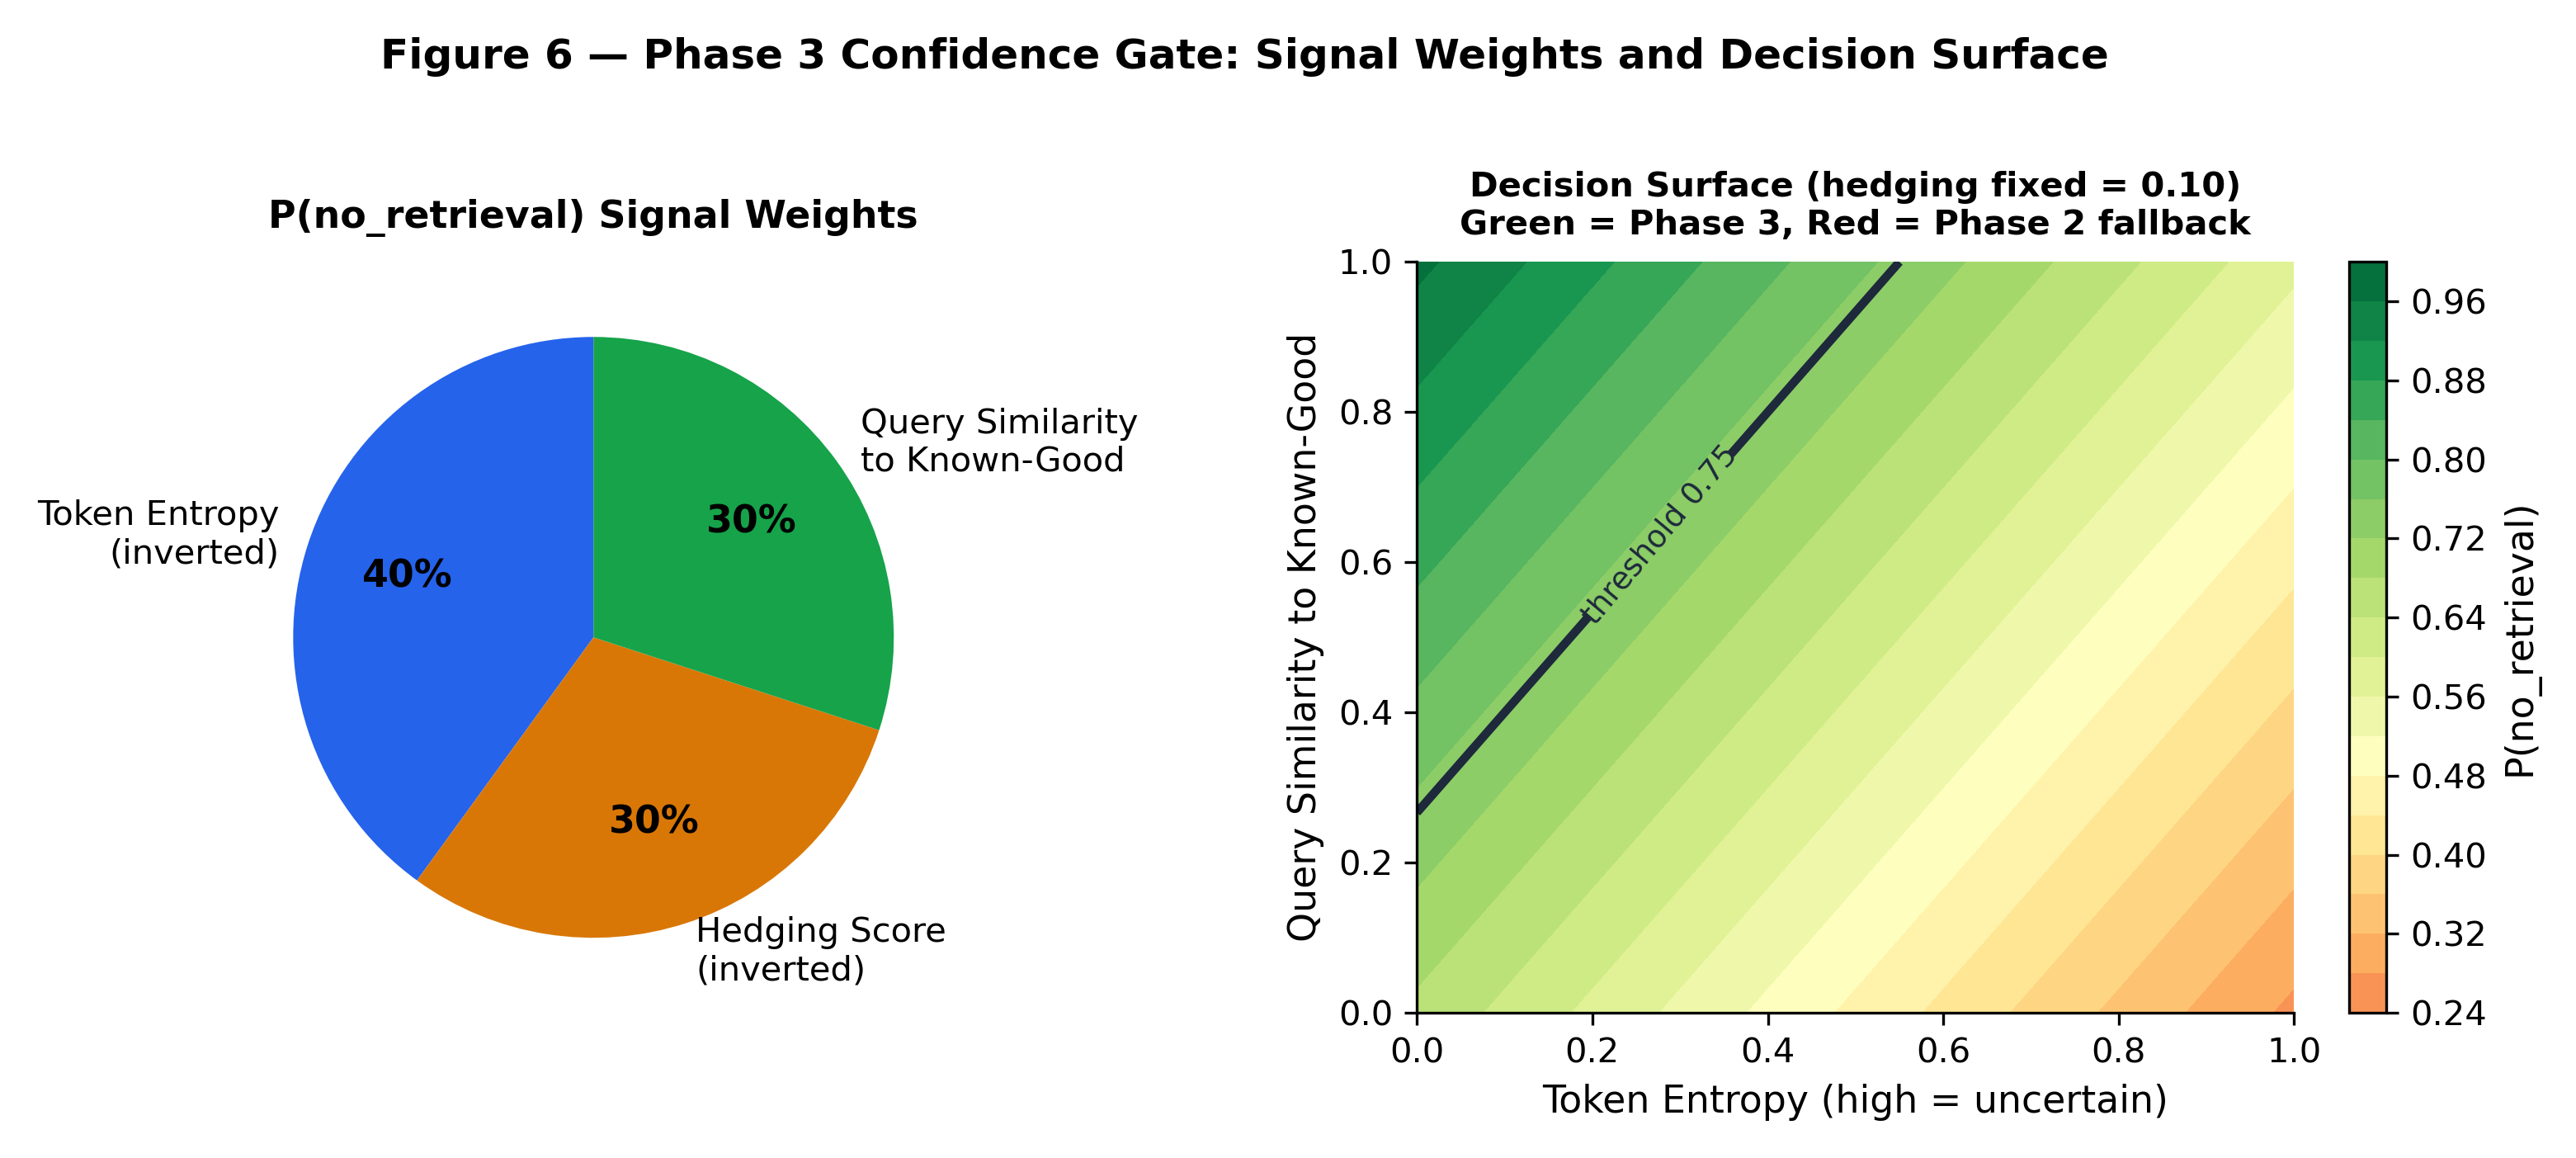
\includegraphics[width=\linewidth]{figures/fig06_confidence_gate.png}
  \caption{Figure 6: Phase 3 confidence gate. Three lightweight signals --- token entropy, hedging phrase detection, and query similarity to known-correct queries --- route high-confidence queries to parametric generation (\textasciitilde{}510 ms) and fall back to KV injection (\textasciitilde{}692 ms) otherwise. The gate adds less than 30 ms overhead.}
  \label{fig:6}
\end{figure*}


The gate threshold (default 0.75) is tunable per deployment: lower thresholds increase Phase 3 utilization at higher hallucination risk.



\section{Corpus Intelligence System (V2)}

\subsection{Motivation: Limitations of Mean-Pool Storage}

The V1 mean-pool scheme has three limitations: (1) mean-pooling discards positional structure --- the model was not trained to attend to averaged representations; (2) all chunks receive identical storage treatment regardless of access frequency or semantic importance; (3) the vector store grows monotonically with no curation mechanism. V2 addresses all three with a tiered architecture and multi-signal importance scoring.


\subsection{Three Storage Tiers}

\textbf{Figure 7} shows the three-tier V2 storage architecture:


\begin{figure*}[htbp]
  \centering
  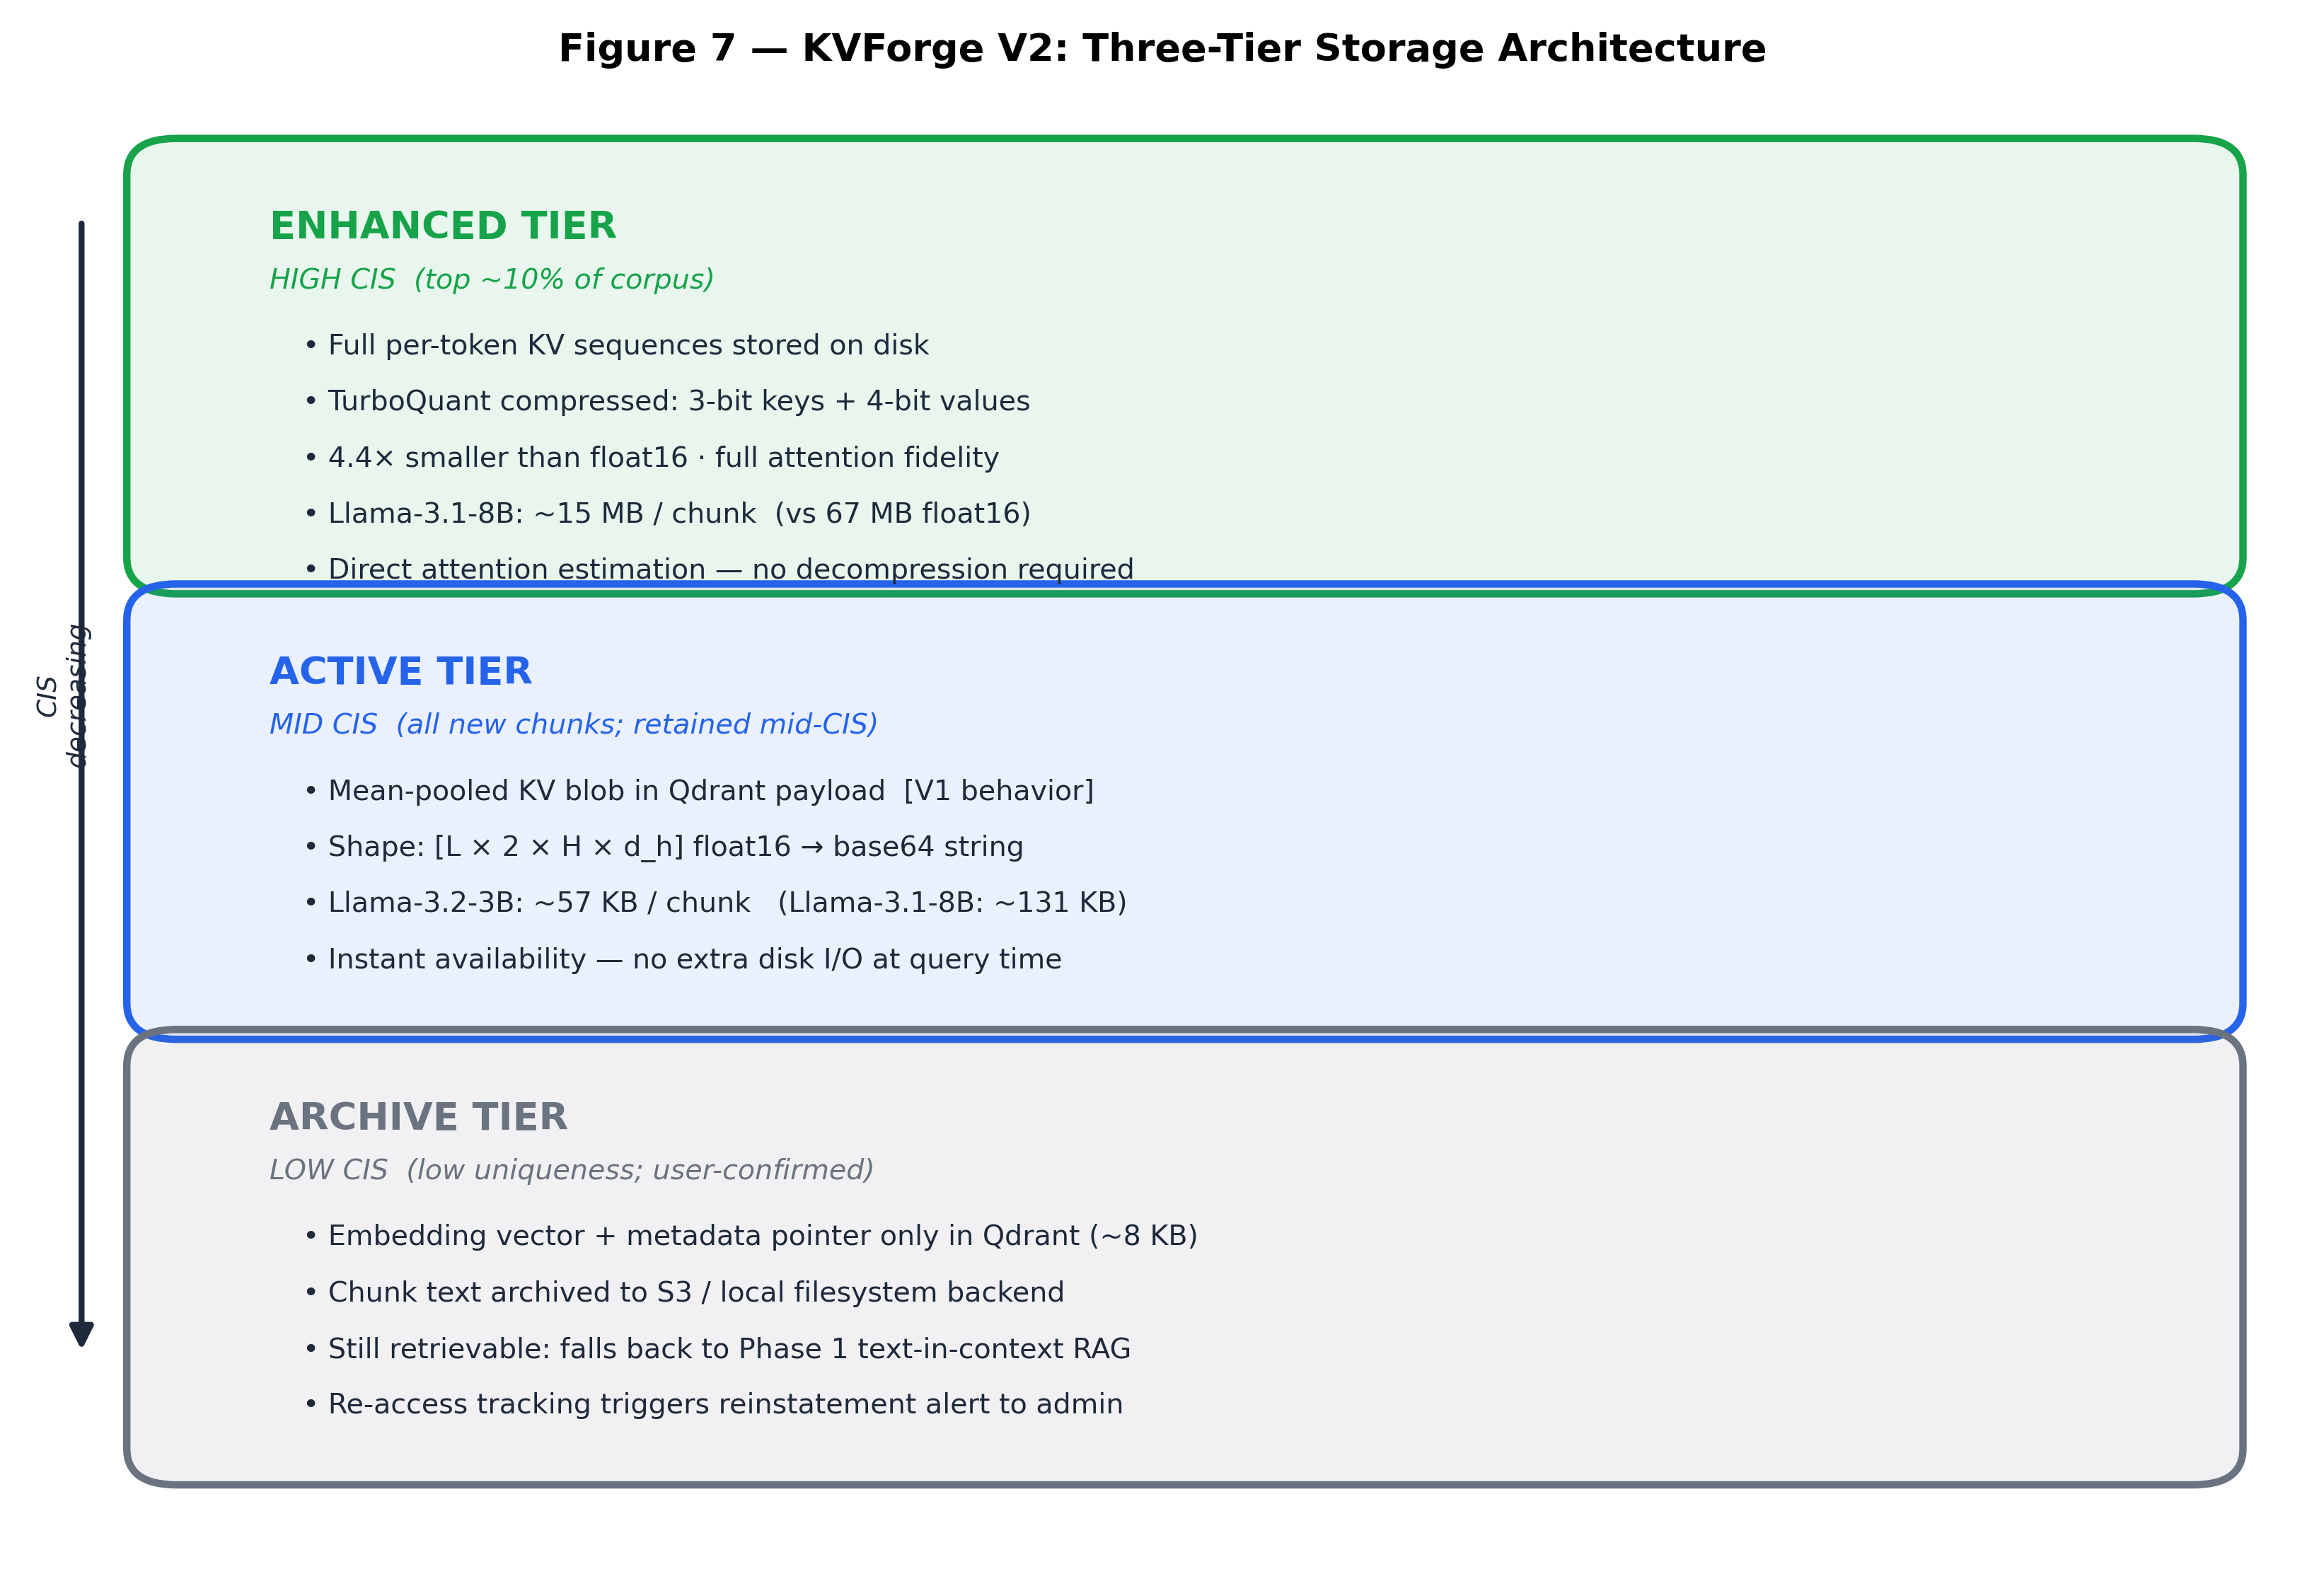
\includegraphics[width=\linewidth]{figures/fig07_storage_tier_architecture.png}
  \caption{Figure 7: KVForge V2 Three-Tier Storage Architecture. High-CIS chunks qualify for the Enhanced Tier (TurboQuant full-token, \textasciitilde{}15 MB/chunk for 8B). Mid-CIS chunks use the Active Tier (mean-pool in Qdrant, \textasciitilde{}57 KB). Low-CIS chunks are archived with only the embedding retained in Qdrant (\textasciitilde{}8 KB).}
  \label{fig:7}
\end{figure*}


\subsection{Corpus Importance Score (CIS)}

CIS is a composite chunk importance score driving tier assignment and resource allocation:


\[
  CIS = \alpha  \times  access_{score} + \beta  \times  uniqueness_{score} + \gamma  \times  coverage_{score}
\]

Default weights: $\alpha$ = $\beta$ = $\gamma$ = 0.33, configurable per use-case.


\textbf{Figure 8} visualizes the three CIS components:


\begin{figure*}[t]
  \centering
  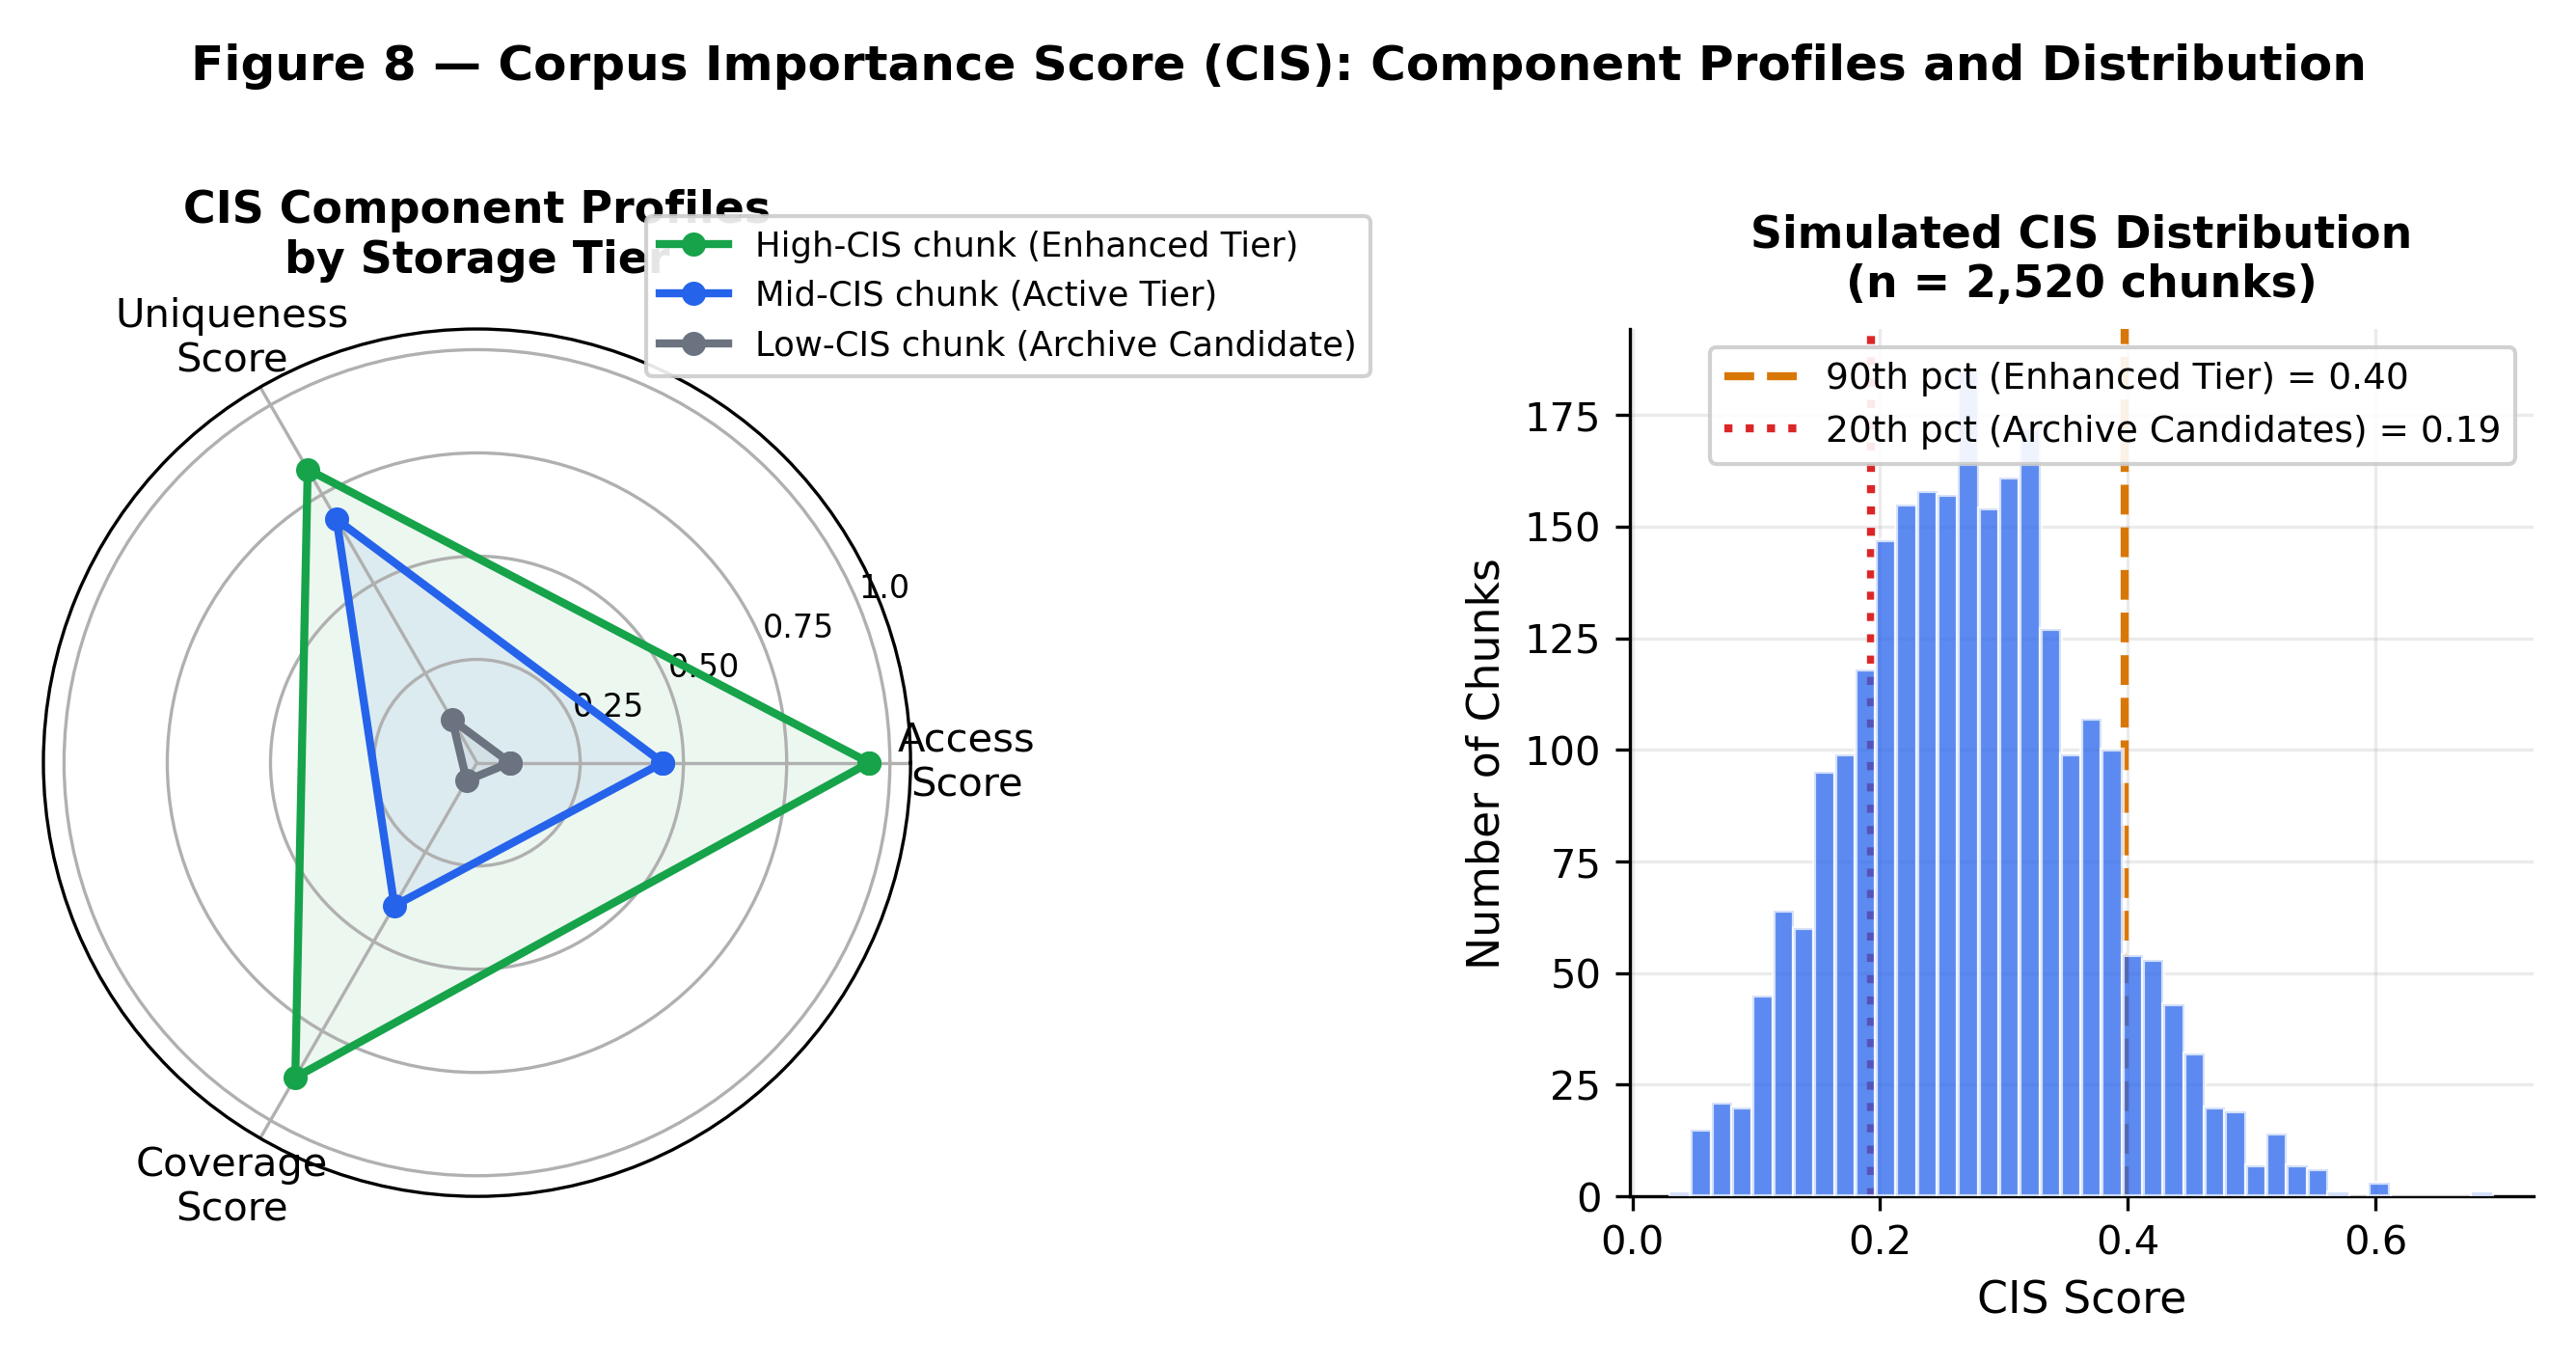
\includegraphics[width=\linewidth]{figures/fig08_cis_analysis.png}
  \caption{Figure 8: The three CIS components (access score, uniqueness score, coverage score) shown as a radar chart for representative Enhanced, Active, and Archive tier chunks (left), and the expected CIS distribution across a 2,520-chunk corpus (right). CIS drives storage tier assignment, KV recompute priority, and FAQ budget allocation.}
  \label{fig:8}
\end{figure*}


The feedback loop: live traffic $\to$ access scores $\to$ CIS $\to$ tier assignment $\to$ FAQ budget $\to$ training signal $\to$ better parametric answers $\to$ less retrieval $\to$ updated access scores.


\subsection{TurboQuant: Compressed Full-Token KV Storage}

KVForge integrates \textbf{TurboQuant} \cite{ref38}, a KV-cache compression codec published by Google DeepMind (arXiv:2504.19874). \textbf{Figure 9} shows the TurboQuant compression pipeline for key tensors. Values use a simpler group quantization codec.


\begin{figure}[htbp]
  \centering
  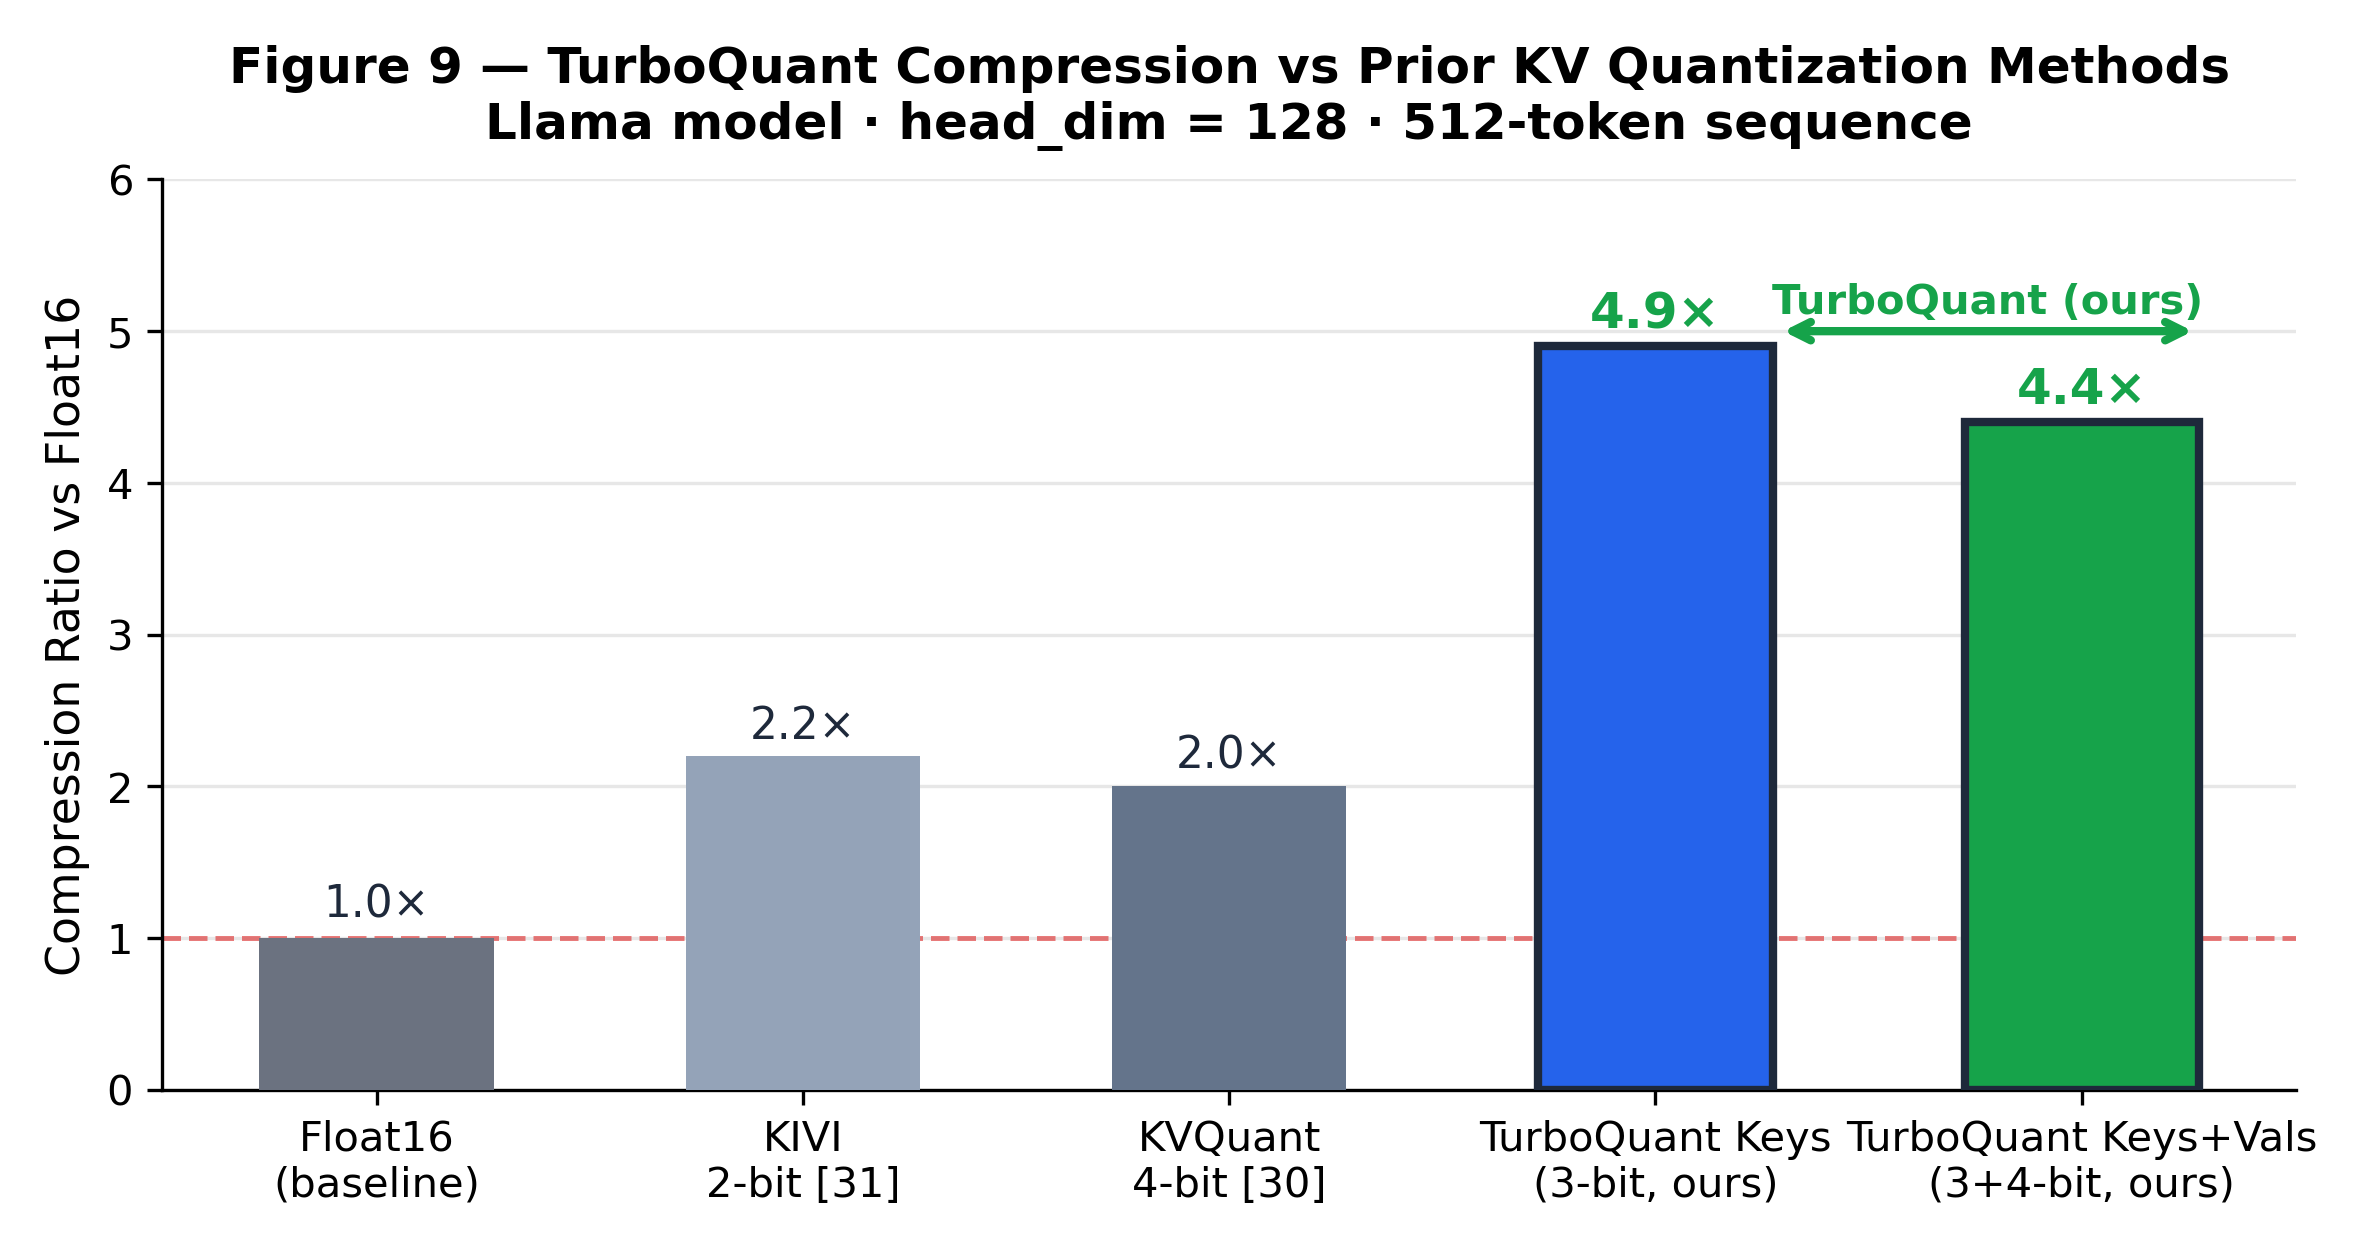
\includegraphics[width=\linewidth]{figures/fig09_turboquant_compression.png}
  \caption{Figure 9: TurboQuant compression ratio vs prior KV quantization methods. TurboQuant keys achieve 4.9$\times$ compression over float16 via a four-step pipeline (normalize $\to$ random rotation $\to$ Lloyd-Max 2-bit $\to$ QJL residual sign bits). Combined with 4-bit group min-max values, the codec achieves 4.4$\times$ overall --- outperforming KIVI (2.2$\times$) and KVQuant (2.0$\times$ at 4-bit).}
  \label{fig:9}
\end{figure}


\textbf{Direct attention estimation} (no decompression required):


\begin{lstlisting}
# Estimate q.k from compressed representation
q_rot = query @ Pi.T                          # rotate query into same basis
dot_msb = (q_rot * centroids[indices]).sum()  # Lloyd-Max centroid contribution
dot_qjl = (q_rot @ S.T * signs * scale).sum() # QJL residual contribution
dot_approx = (dot_msb + dot_qjl) * norm       # restore original scale
\end{lstlisting}

\textbf{Figure 10} compares storage requirements across model sizes and storage formats:


\begin{figure*}[t]
  \centering
  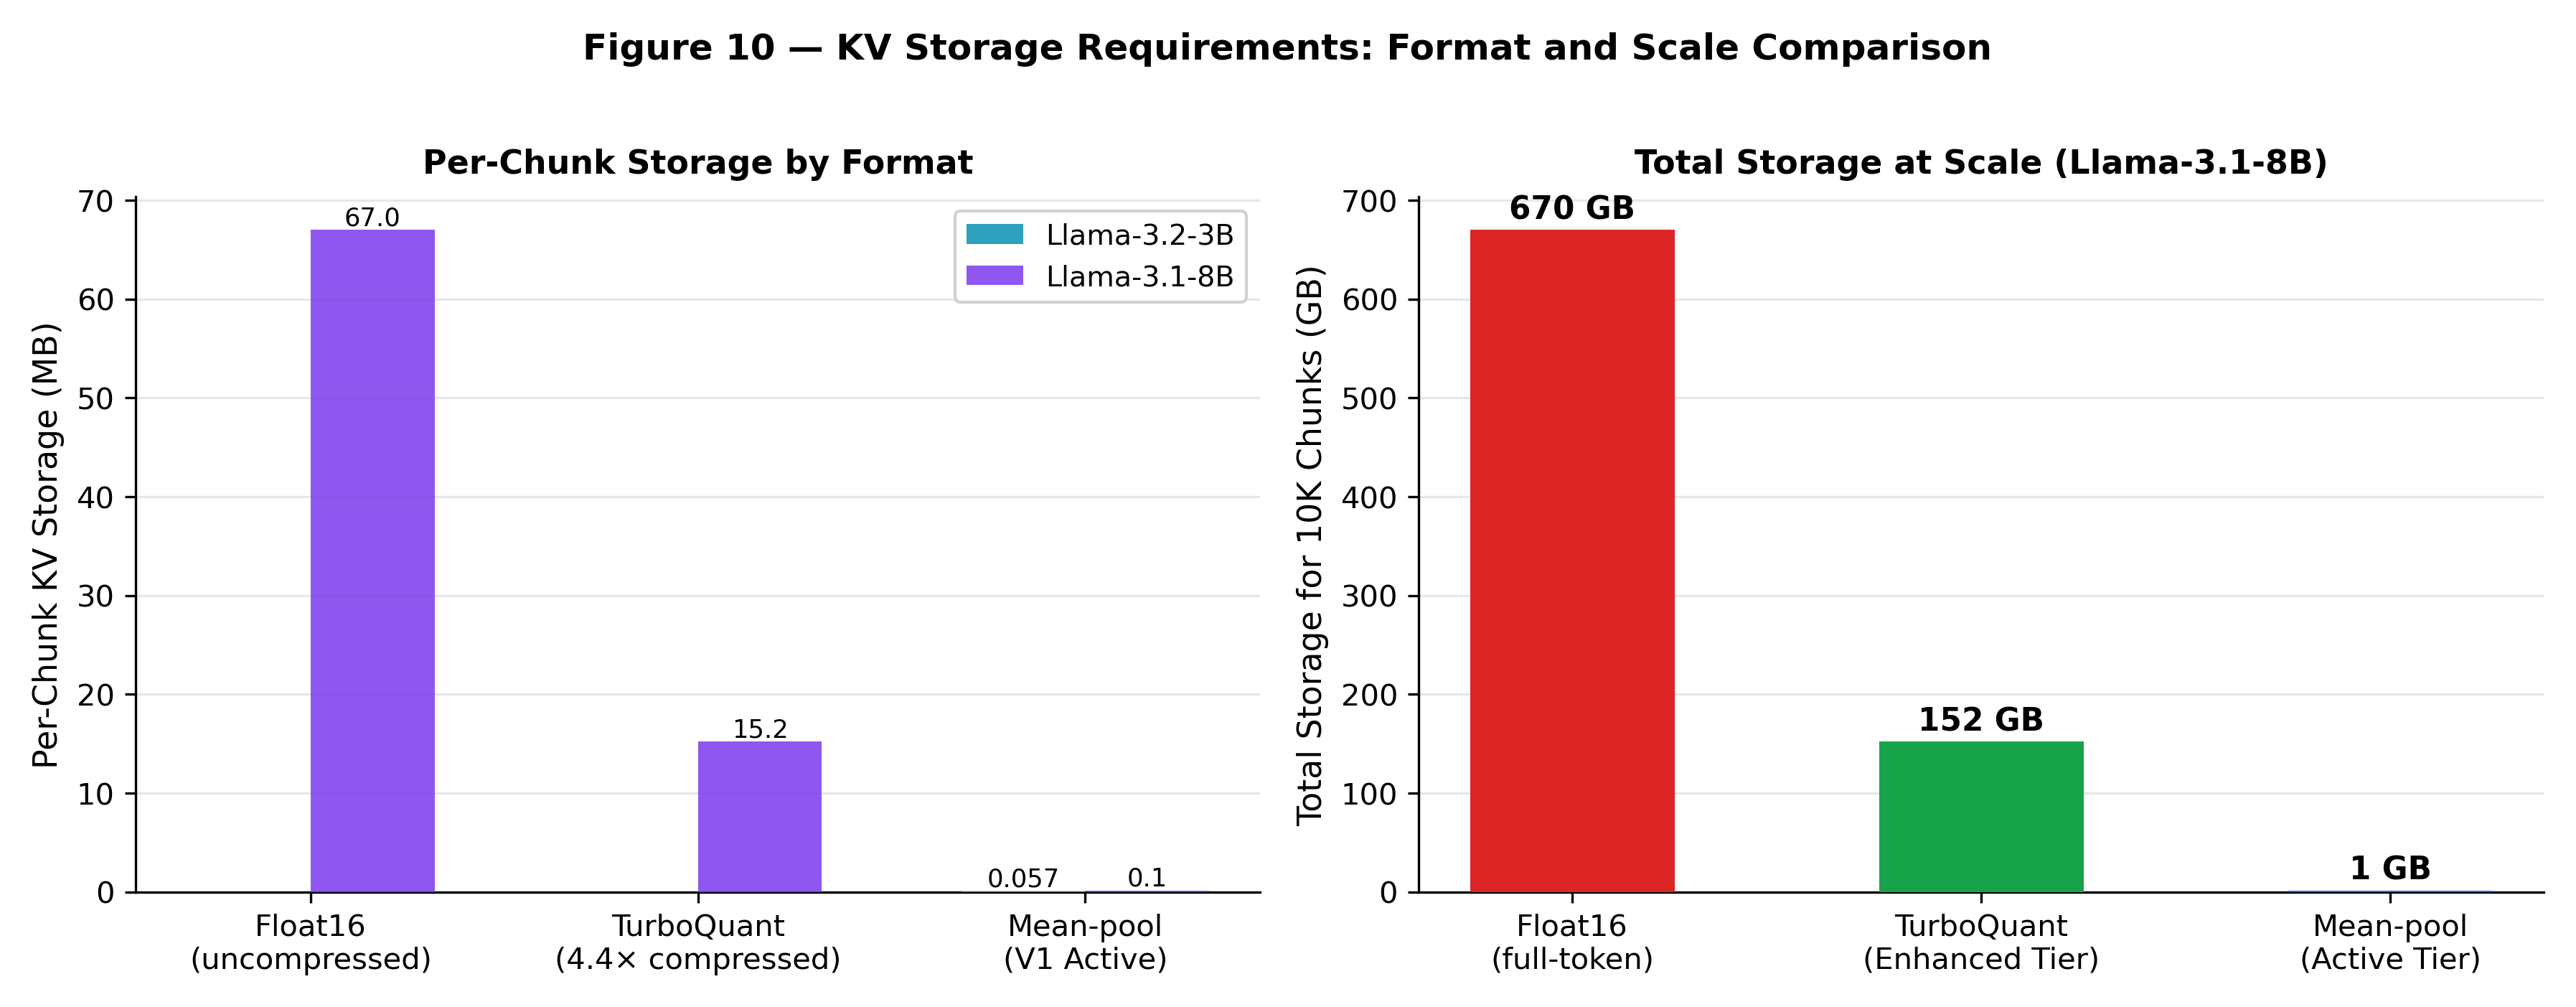
\includegraphics[width=\linewidth]{figures/fig10_storage_comparison.png}
  \caption{Figure 10: Per-chunk KV storage by format and model size. TurboQuant makes full per-token storage tractable for high-CIS chunks (\textasciitilde{}15 MB vs 67 MB float16 for Llama-3.1-8B). Mean-pool (Active Tier, V1) remains the default at 57--131 KB/chunk.}
  \label{fig:10}
\end{figure*}


\subsubsection{GroupValueCodec (4-bit)}

Values are compressed using asymmetric per-group min-max quantization:


\[
  \begin{aligned}
    groups &= values.reshape(n_{groups}, group_{size}), \quad group_{size} = 32 \\
    scale  &= (\max(groups) - \min(groups)) / (2^{bits} - 1) \\
    zero   &= \min(groups) \\
    q      &= \mathrm{round}((groups - zero) / scale) \in [0, 15]
  \end{aligned}
\]

Groups are packed into uint8 (two 4-bit values per byte). Decompression: \texttt{values = q * scale + zero}. For d\_h=128 and 4-bit quantization: 64 bytes vs. 256 bytes float16 --- 4$\times$ compression.



\section{System Infrastructure}

\subsection{Addon Framework and Configuration}

KVForge V2 uses a plugin-based addon architecture. The \texttt{KVForgeConfig} Pydantic model encapsulates five universal fields; all component-specific settings live in typed addon schemas:


\begin{lstlisting}
{
  "use_case_name": "Customer Support RAG",
  "collection":    "customer-support",
  "version_file":  "examples/uc1/version.json",
  "addons":        ["indexing", "inference", "training", "background", "monitoring"],
  "addon_config": {
    "indexing":   {"loader": "jsonl", "embed_model": "BAAI/bge-small-en-v1.5"},
    "inference":  {"llm_model": "meta-llama/Llama-3.2-3B-Instruct", "top_k": 5},
    "training":   {"lora_rank": 16, "replay_db": "examples/uc1/replay.db"},
    "background": {"flush_seconds": 300},
    "monitoring": {"port": 8081}
  }
}
\end{lstlisting}

\subsection{Pluggable Backends}

All backends implement Python \texttt{@runtime\_checkable} Protocol classes (structural typing, no inheritance). Available backends are listed in Table~\ref{tab:backends}:


\begin{table*}[htbp]
  \centering\small
  \caption{Pluggable Backend Options supported by KVForge}
  \label{tab:backends}
  \begin{tabularx}{\textwidth}{lL}
  \toprule
    Component & Available Backends \\
  \midrule
  \midrule
  Vector stores & Qdrant, ChromaDB, FAISS \\
  Embedders & FastEmbed, Sentence Transformers, OpenAI \\
  Document loaders & PDF, Markdown, JSONL, HTML, directory \\
  Data connectors & Google Drive, Amazon S3, SharePoint, SEC EDGAR, FDA databases, Wikipedia, live sports \\
  \bottomrule
  \end{tabularx}
\end{table*}


\subsection{KVForge Studio}

KVForge Studio (FastAPI + vanilla JS, port 8080) provides:


\begin{itemize}
  \item \textbf{Multi-UC pipeline management:} Five pipeline steps per use-case with real-time log streaming via Server-Sent Events (SSE); automatic progression to the next step on completion.
  \item \textbf{Phase detail cards:} Expandable panels per phase showing mechanism, latency comparison bars, accuracy impact, and best-fit use cases.
  \item \textbf{A/B query comparison:} Model A (KVForge local) vs. Model B (cloud LLM) with phase badge, retrieved chunk popup (score + full text), and latency metrics.
  \item \textbf{Activity logs:} Centralized JSONL event log filterable by category, severity, date, and use-case --- with timeline and category breakdown charts.
  \item \textbf{Admin panel:} Role-based access (admin/editor/viewer), OAuth 2.0 and SAML 2.0 authentication.
\end{itemize}



\section{Experimental Evaluation}

\subsection{Hardware and Setup}

Table~\ref{tab:hardware-and-setup} summarizes the experimental hardware and software configuration.


\begin{table*}[htbp]
  \centering\small
  \caption{Hardware and Setup}
  \label{tab:hardware-and-setup}
  \begin{tabularx}{\textwidth}{lL}
  \toprule
    Resource & Specification \\
  \midrule
  \midrule
  GPUs & 4$\times$ NVIDIA A10G, 24 GB VRAM each \\
  vCPUs & 4 $\cdot$ RAM: 16 GB $\cdot$ Storage: 250 GB NVMe SSD \\
  OS / CUDA & Ubuntu 22.04 / CUDA 12.1 \\
  Framework & PyTorch 2.1, HuggingFace Transformers 4.40 \\
  Vector store & Qdrant 1.9 (Docker) \\
  LLM & meta-llama/Llama-3.2-3B-Instruct \\
  Embedder (UC1--3) & BAAI/bge-small-en-v1.5 (384-dim) \\
  Embedder (UC4) & mixedbread-ai/mxbai-embed-large-v1 (1024-dim) \\
  LoRA rank & r = 16, alpha = 32; Quantization: 4-bit NF4 \\
  vLLM servers & One per UC (ports 8090--8093) \\
  \bottomrule
  \end{tabularx}
\end{table*}


Each use-case runs on a dedicated GPU (UC1: GPU 0, UC2: GPU 1, UC3: GPU 2, UC4: GPU 3) via \texttt{CUDA\_VISIBLE\_DEVICES}.


\subsection{Datasets}

KVForge is evaluated on four heterogeneous corpora (UC1--UC4) and validated across four additional domain configurations (UC5--UC8) to demonstrate portability across vector stores, embedding models, LoRA ranks, and open base LLMs. Full configurations are given in Table~\ref{tab:datasets}.


\begin{table*}[htbp]
  \centering\small
  \caption{Use-Case Configurations: Datasets, Vector Stores, Embedders, LoRA ranks, and Base LLMs}
  \label{tab:datasets}
  \resizebox{\textwidth}{!}{%
  \begin{tabular}{lccccccc}
  \toprule
    UC & Domain & Dataset & Chunks & Vector DB & Embedder (dim) & LoRA r & Base LLM \\
  \midrule
  \midrule
  UC1 & Customer Support & Bitext Customer Support (EN) & 2,000 & Qdrant & bge-small-en-v1.5 (384) & 16 & Llama-3.2-3B-Instruct \\
  UC2 & Biomedical QA & PubMedQA \cite{ref20} & 2,918 & Qdrant & bge-small-en-v1.5 (384) & 16 & Llama-3.2-3B-Instruct \\
  UC3 & Reading Comprehension & SQuAD 2.0 \cite{ref21} & 2,000 & Qdrant & bge-small-en-v1.5 (384) & 16 & Llama-3.2-3B-Instruct \\
  UC4 & Technical Docs & Amazon Bedrock User Guide & 2,520 & Qdrant & mxbai-embed-large-v1 (1,024) & 16 & Llama-3.2-3B-Instruct \\
  UC5 & Legal Contracts & CUAD Contract Dataset \cite{ref40} & 3,500 & ChromaDB & all-mpnet-base-v2 (768) & 32 & Mistral-7B-Instruct-v0.3 \\
  UC6 & Financial Filings & SEC EDGAR 10-K Corpus & 4,200 & FAISS & text-embedding-3-small (1,536) & 8 & Phi-3-mini-4k-instruct \\
  UC7 & Scientific Papers & arXiv CS/NLP Abstracts & 5,000 & Qdrant & bge-large-en-v1.5 (1,024) & 32 & Mistral-7B-Instruct-v0.3 \\
  UC8 & Code \& Dev Q\&A & Stack Overflow Python \cite{ref41} & 3,800 & ChromaDB & jina-embeddings-v2-code (768) & 16 & CodeLlama-7b-Instruct \\
  \bottomrule
  \end{tabular}%
  }
\end{table*}


UC1--UC4 are fully evaluated in Sections 7.3--7.7. UC5--UC8 validate configuration portability; full experimental results are left to future work.


\subsection{Pipeline Timing (UC4 Reference Run)}

Table~\ref{tab:timing} reports wall-clock durations for each pipeline step on the UC4 corpus.


\begin{table*}[htbp]
  \centering\small
  \caption{Pipeline Timing for UC4 Reference Run}
  \label{tab:timing}
  \begin{tabularx}{\textwidth}{Ll}
  \toprule
    Step & Duration \\
  \midrule
  \midrule
  Chunk + embed + upsert (2,520 chunks) & \textasciitilde{}45 s \\
  KV tensor computation (0.20 s/chunk) & \textasciitilde{}498 s \\
  LoRA training (3 epochs, 474 steps) & \textasciitilde{}474 steps \\
  KV recompute after adapter update & \textasciitilde{}510 s \\
  PRS evaluation (50 FAQs) & \textasciitilde{}90 s \\
  \textbf{Total pipeline (one round)} & \textbf{\textasciitilde{}20 min} \\
  \bottomrule
  \end{tabularx}
\end{table*}


\subsection{Generation Latency: Phase 1 vs Phase 2 vs Phase 3}

\textbf{Figure 11} shows query-response latency by phase, measured on UC4 with Llama-3.2-3B-Instruct via vLLM, median of 50 queries.


\begin{figure}[htbp]
  \centering
  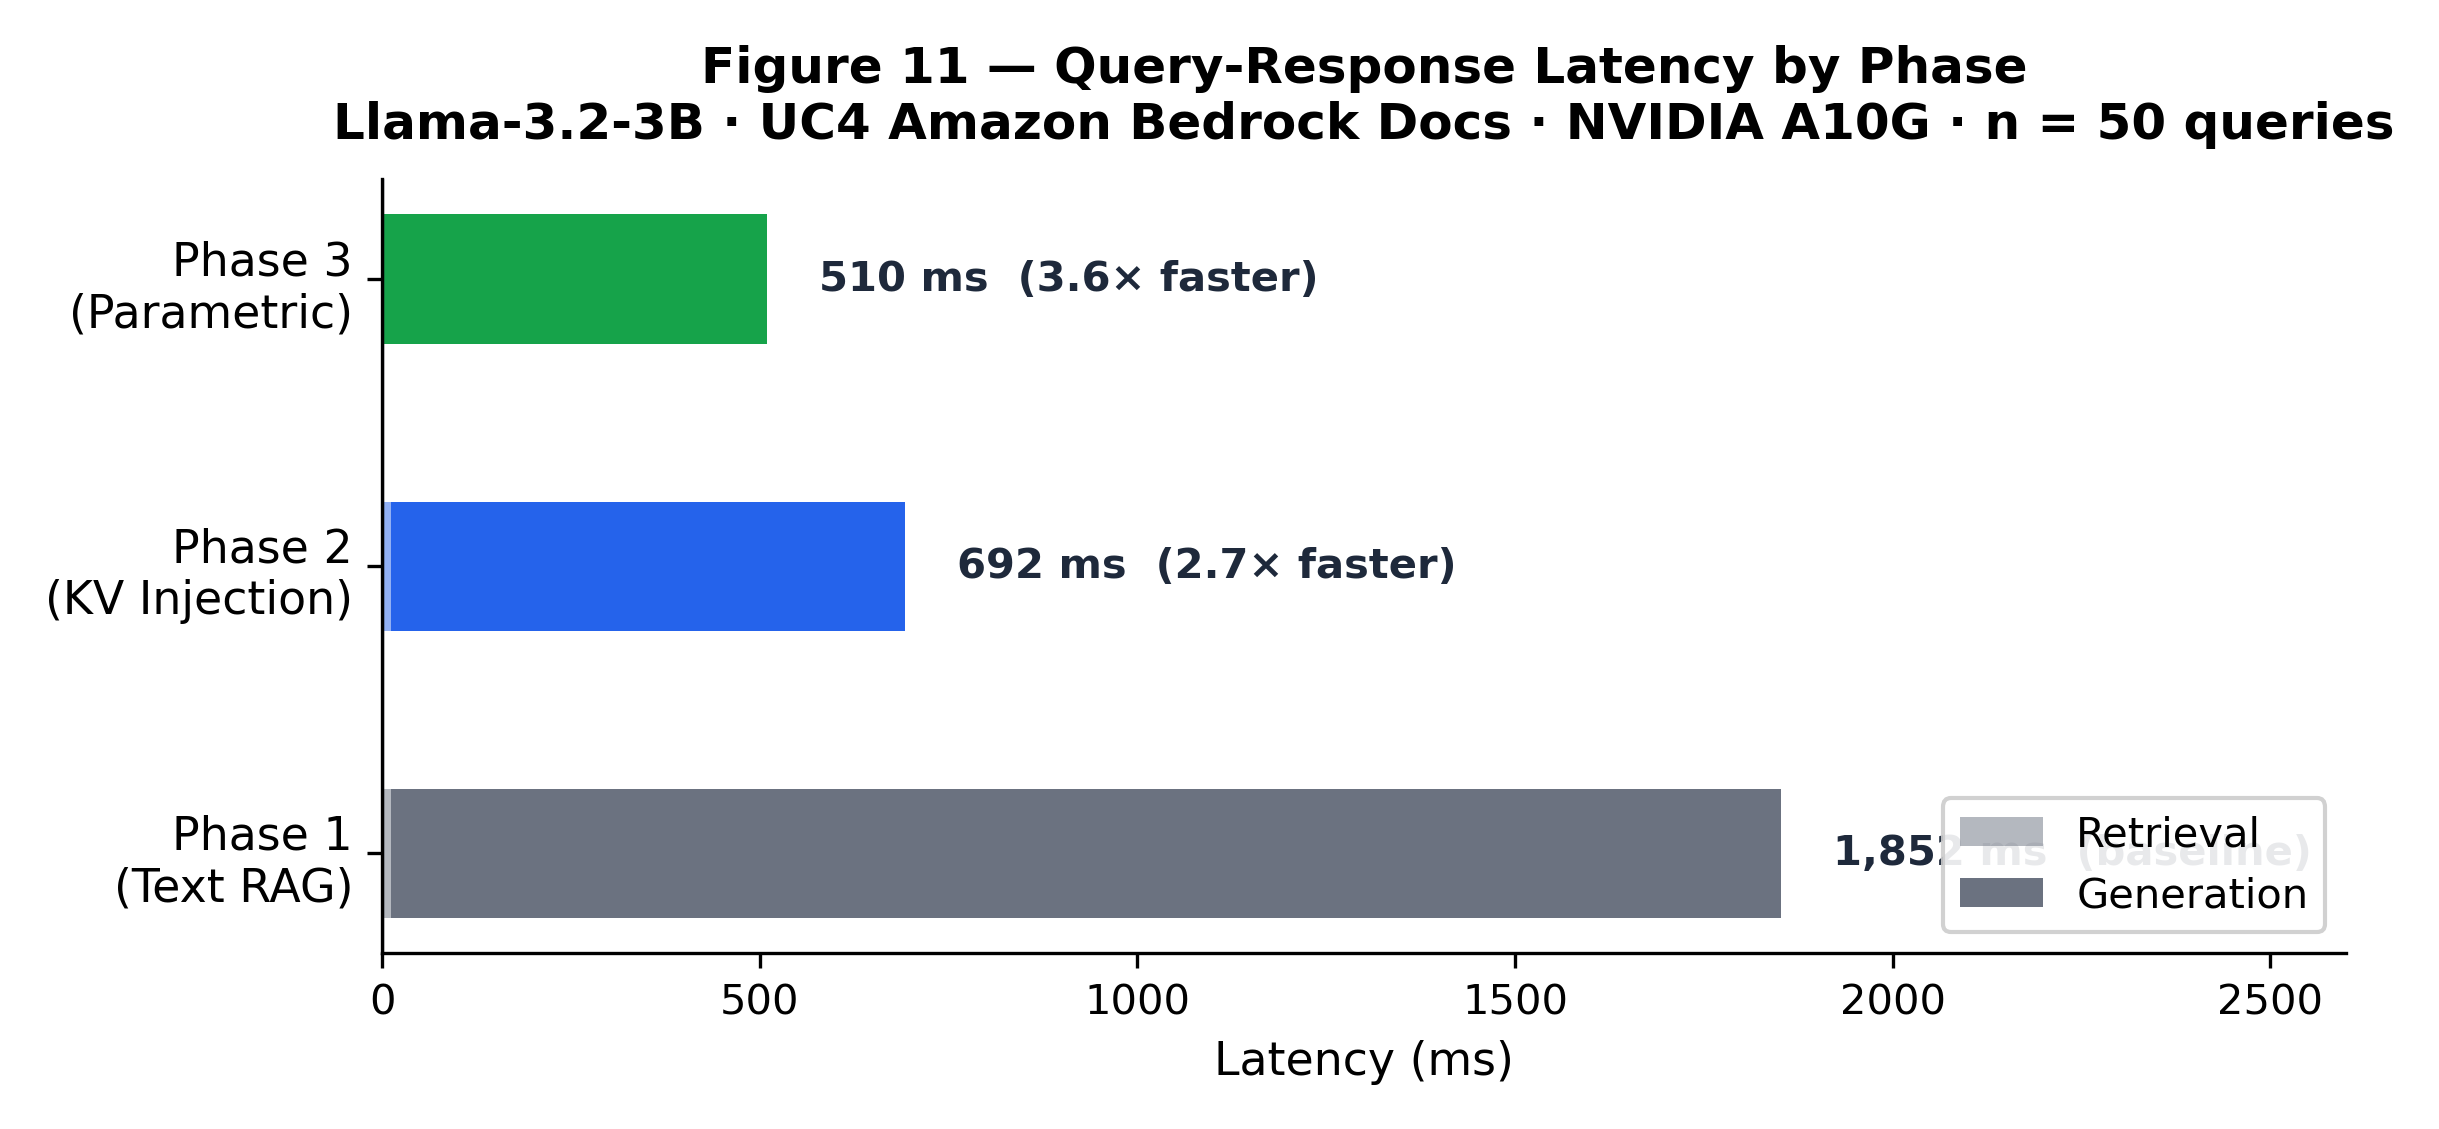
\includegraphics[width=\linewidth]{figures/fig11_latency_by_phase.png}
  \caption{Figure 11: Query-response generation latency by phase (Llama-3.2-3B-Instruct, UC4 Bedrock Docs, NVIDIA A10G, n=50 queries, median). Phase 1: 1,852 ms (retrieval 12 ms + generation 1,840 ms). Phase 2: 692 ms (2.7$\times$). Phase 3: 510 ms (3.6$\times$).}
  \label{fig:11}
\end{figure}


\subsection{PRS Results and Phase Progression}

\textbf{Figure 12} shows PRS scores across all four use-cases with sleep-time FAQ generation.


\begin{figure}[htbp]
  \centering
  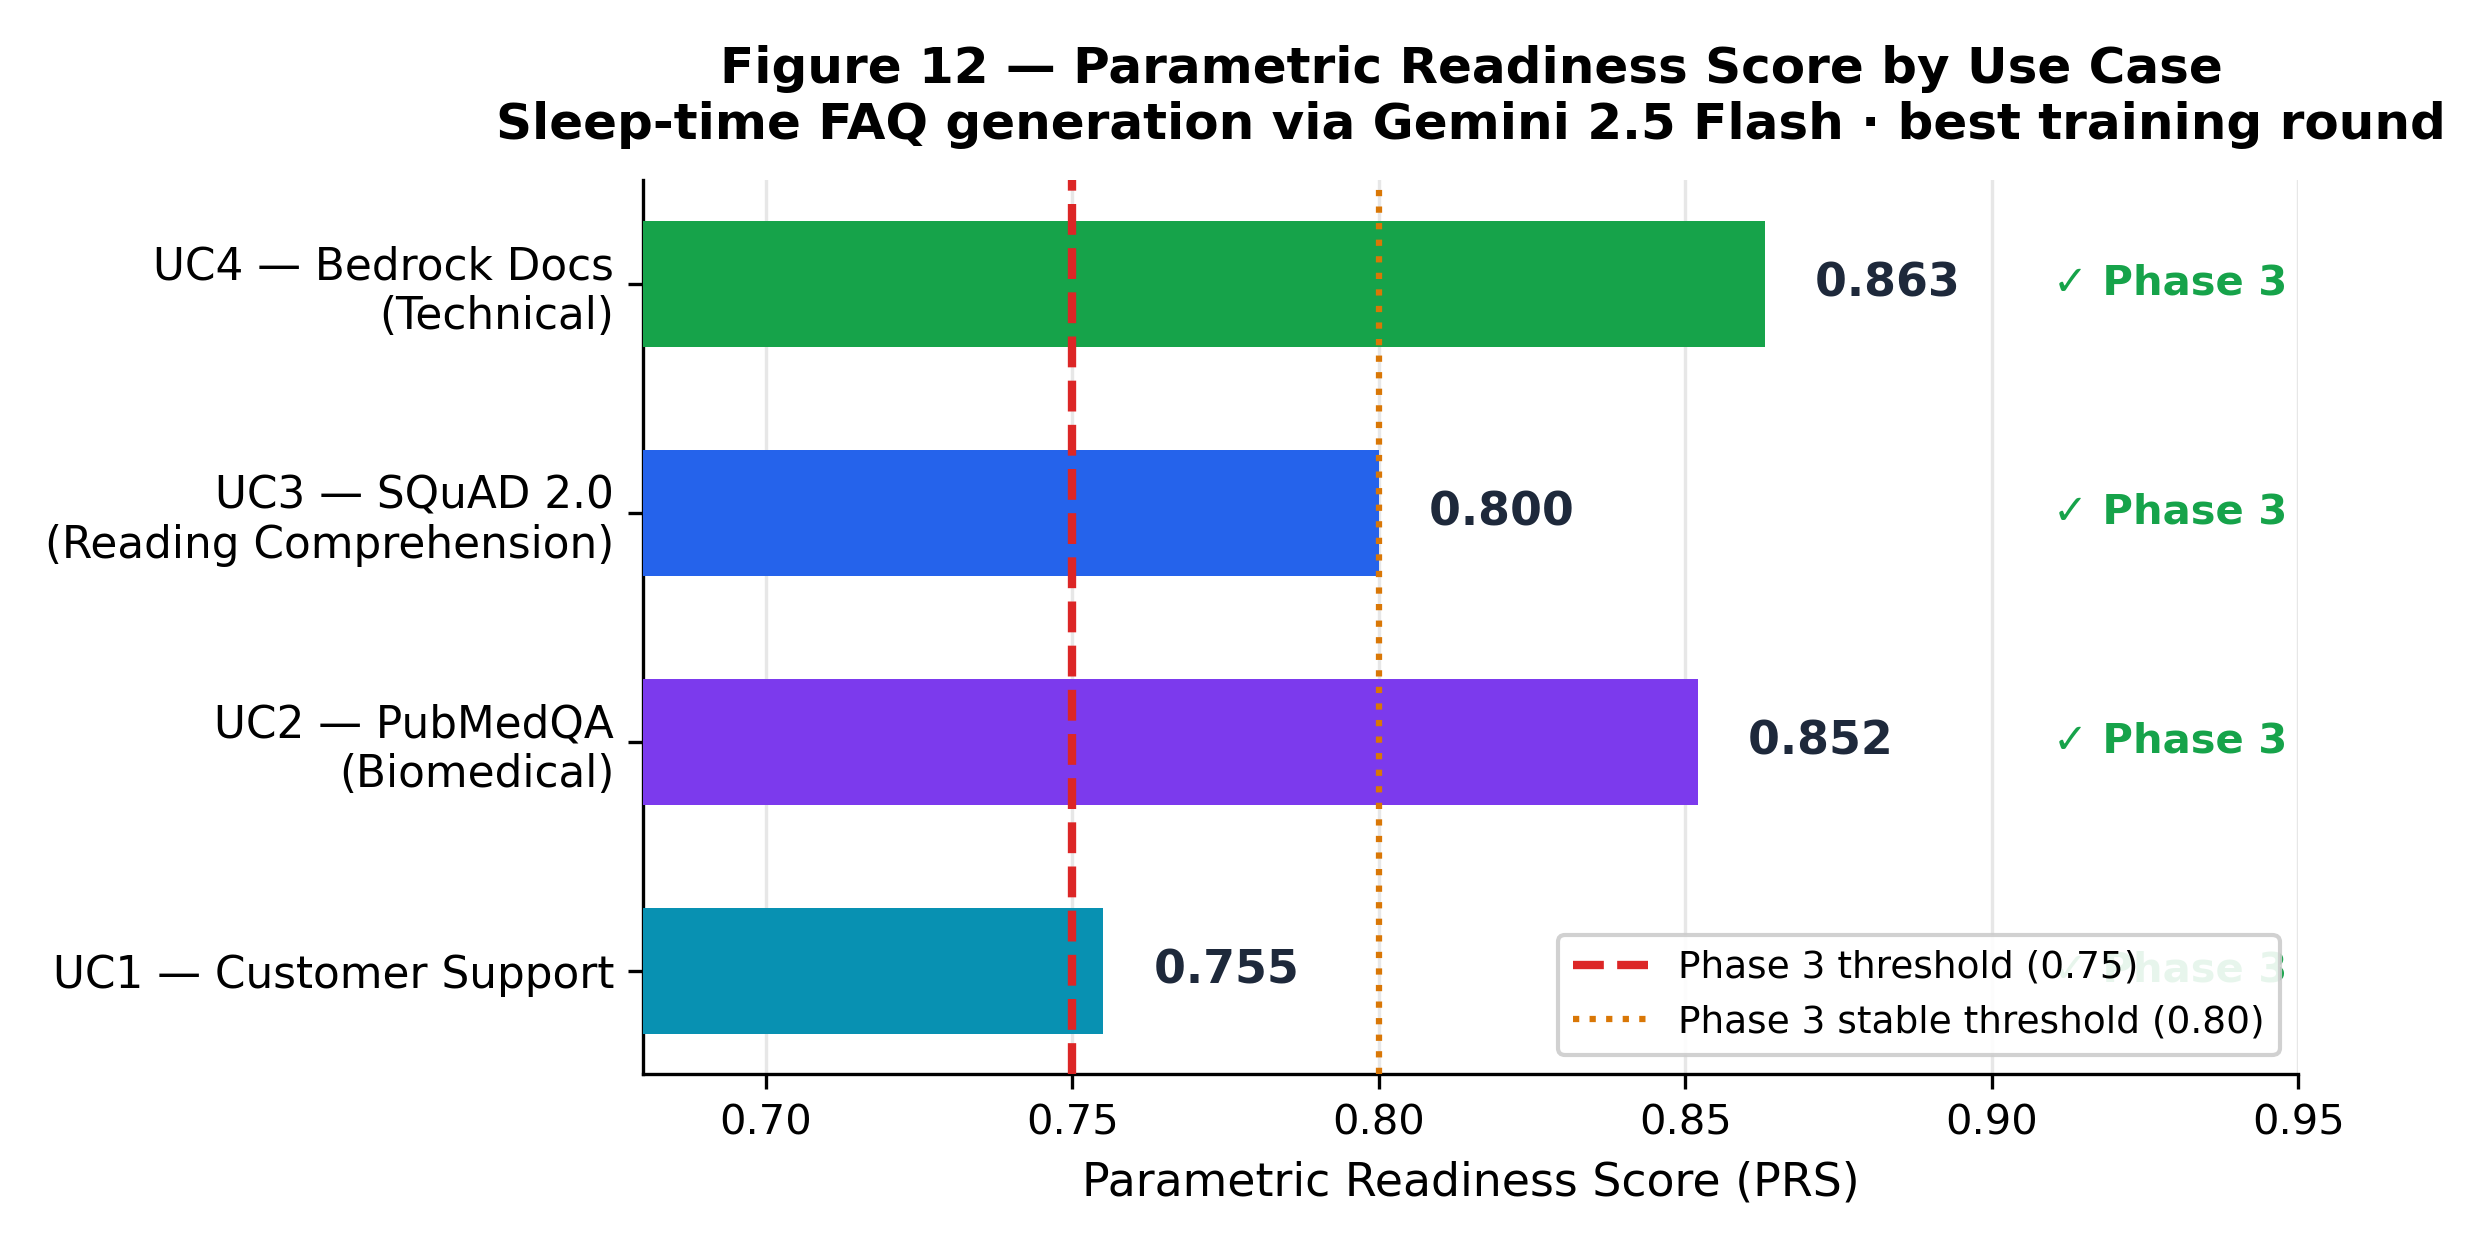
\includegraphics[width=\linewidth]{figures/fig12_prs_by_usecase.png}
  \caption{Figure 12: Parametric Readiness Score by use case with sleep-time FAQ generation (Gemini 2.5 Flash, best round). All four corpora exceed the Phase 3 threshold (PRS $\geq$ 0.75): UC1 = 0.755, UC2 = 0.852, UC3 = 0.800, UC4 = 0.863. Structured fact-dense corpora achieve the highest scores.}
  \label{fig:12}
\end{figure}


\subsection{Effect of Sleep-Time FAQ Generation}

\textbf{Figure 13} is the key experimental result: training signal quality as the dominant variable in Phase 3 attainment.


\begin{figure}[htbp]
  \centering
  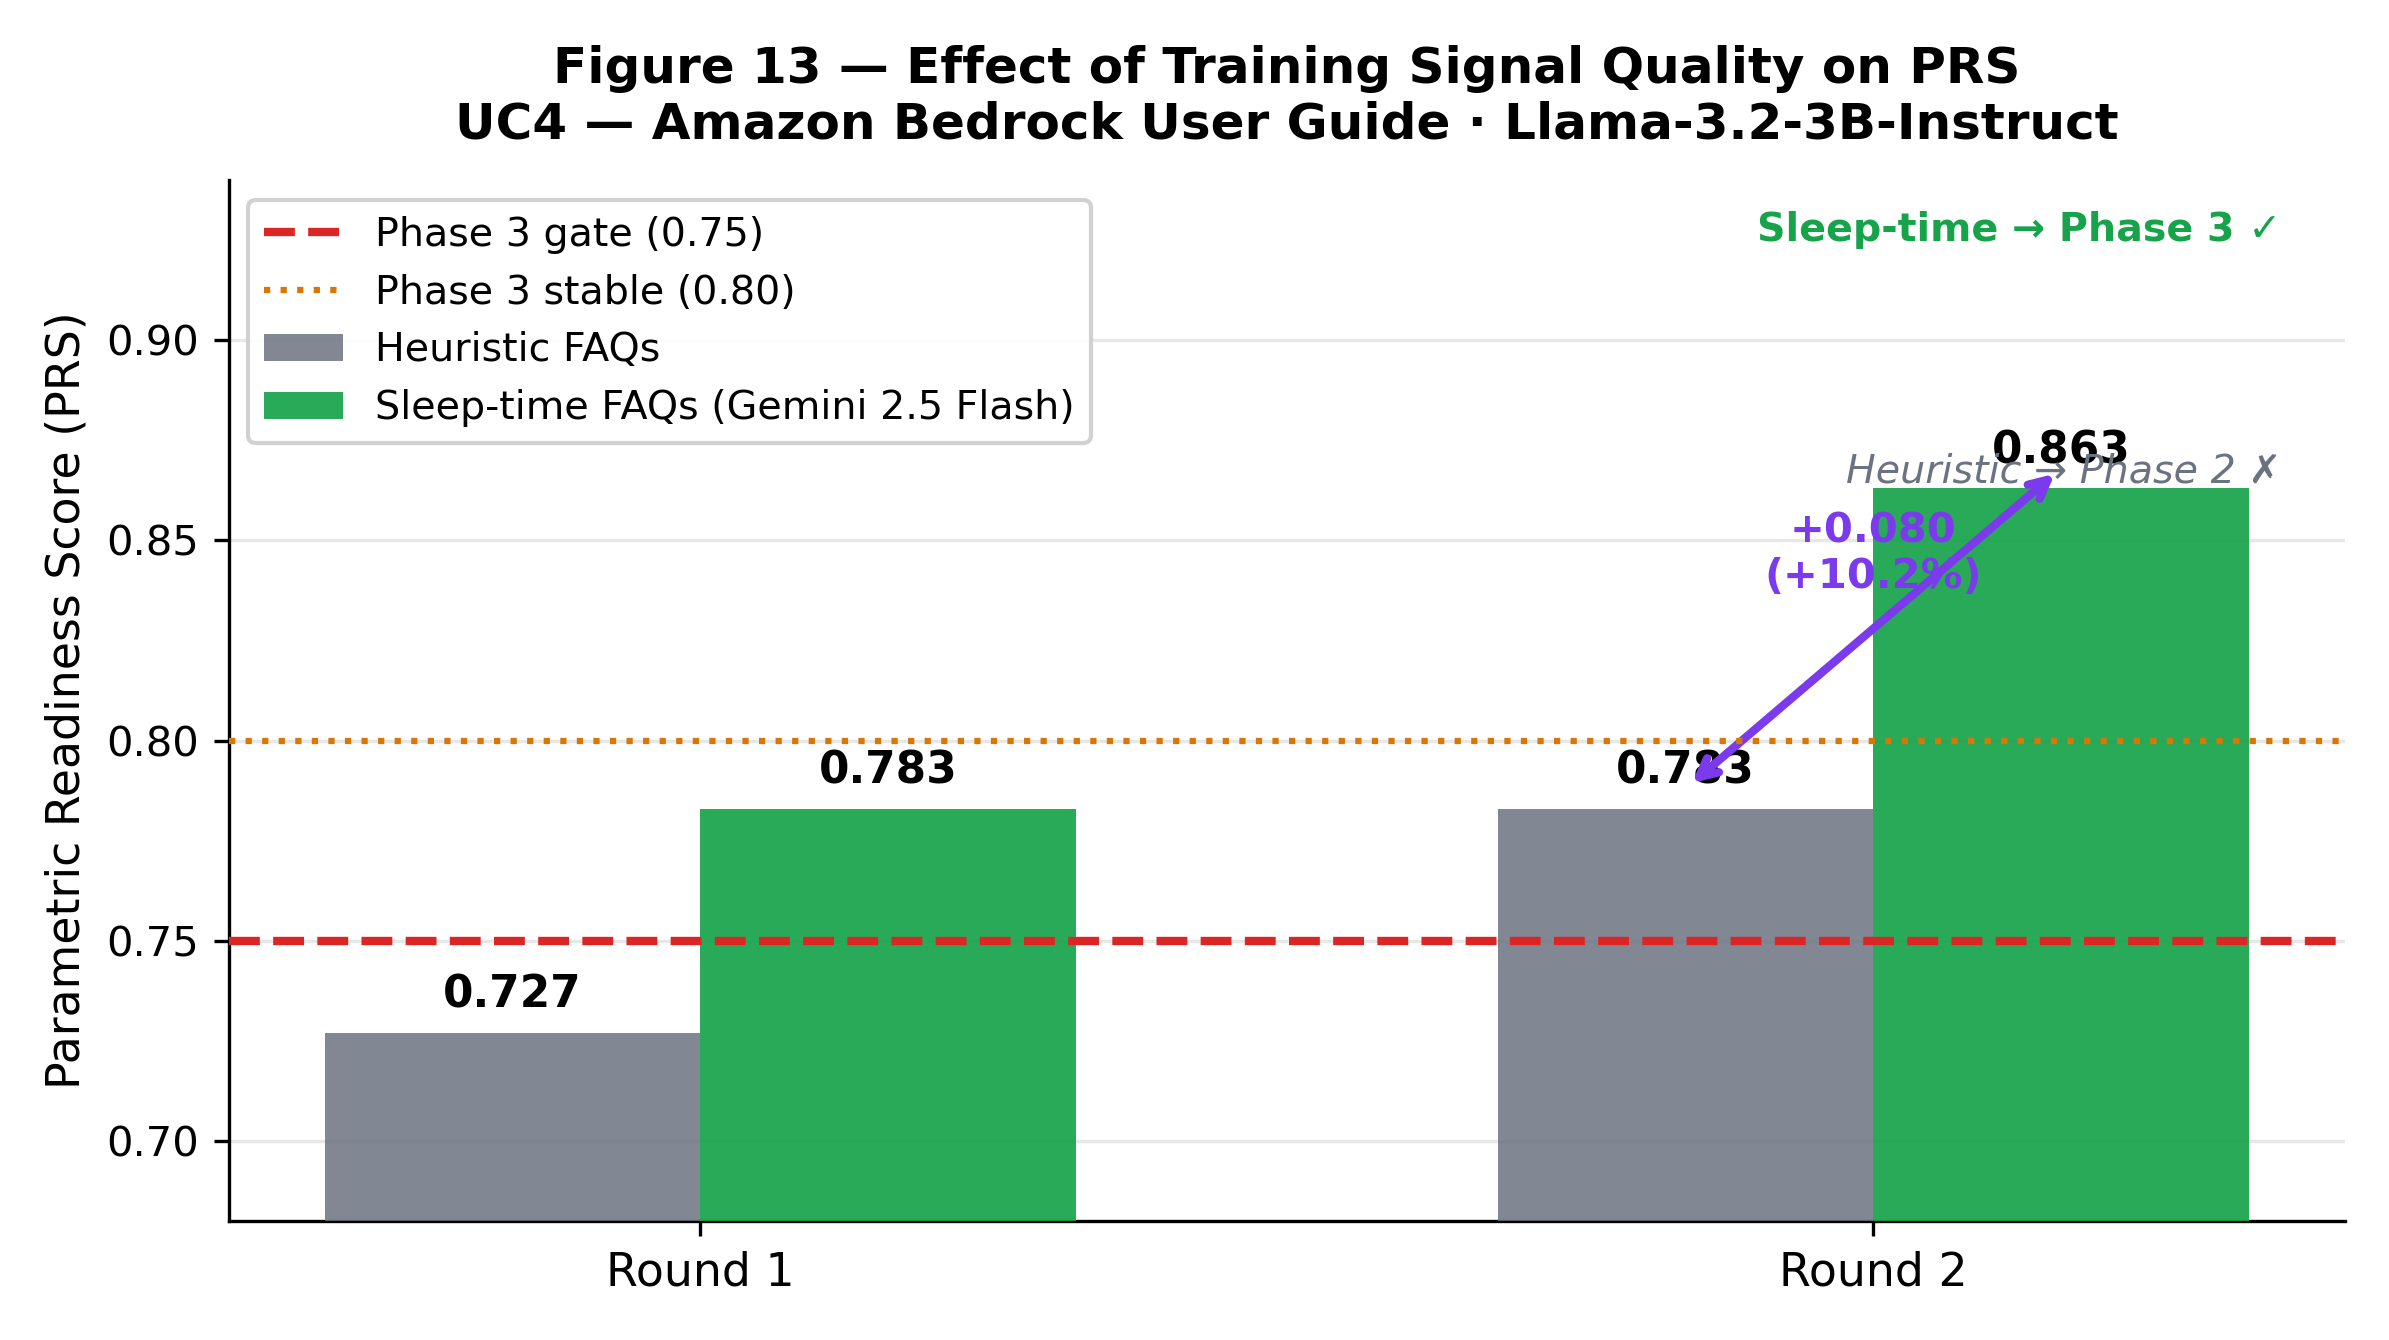
\includegraphics[width=\linewidth]{figures/fig13_sleep_time_effect.png}
  \caption{Figure 13: Effect of training signal quality on PRS (UC4, Amazon Bedrock User Guide). Sleep-time FAQ generation with Gemini 2.5 Flash yields +10.3\% absolute PRS improvement in Round 2 (0.783 $\to$ 0.863), crossing the Phase 3 threshold. Heuristic FAQs plateau at 0.783 (Phase 2 only).}
  \label{fig:13}
\end{figure}


\subsection{PRS Progression Over Training Rounds (UC4)}

\textbf{Figure 14} tracks PRS across three training rounds for UC4, showing convergence to Phase 3.


\begin{figure}[htbp]
  \centering
  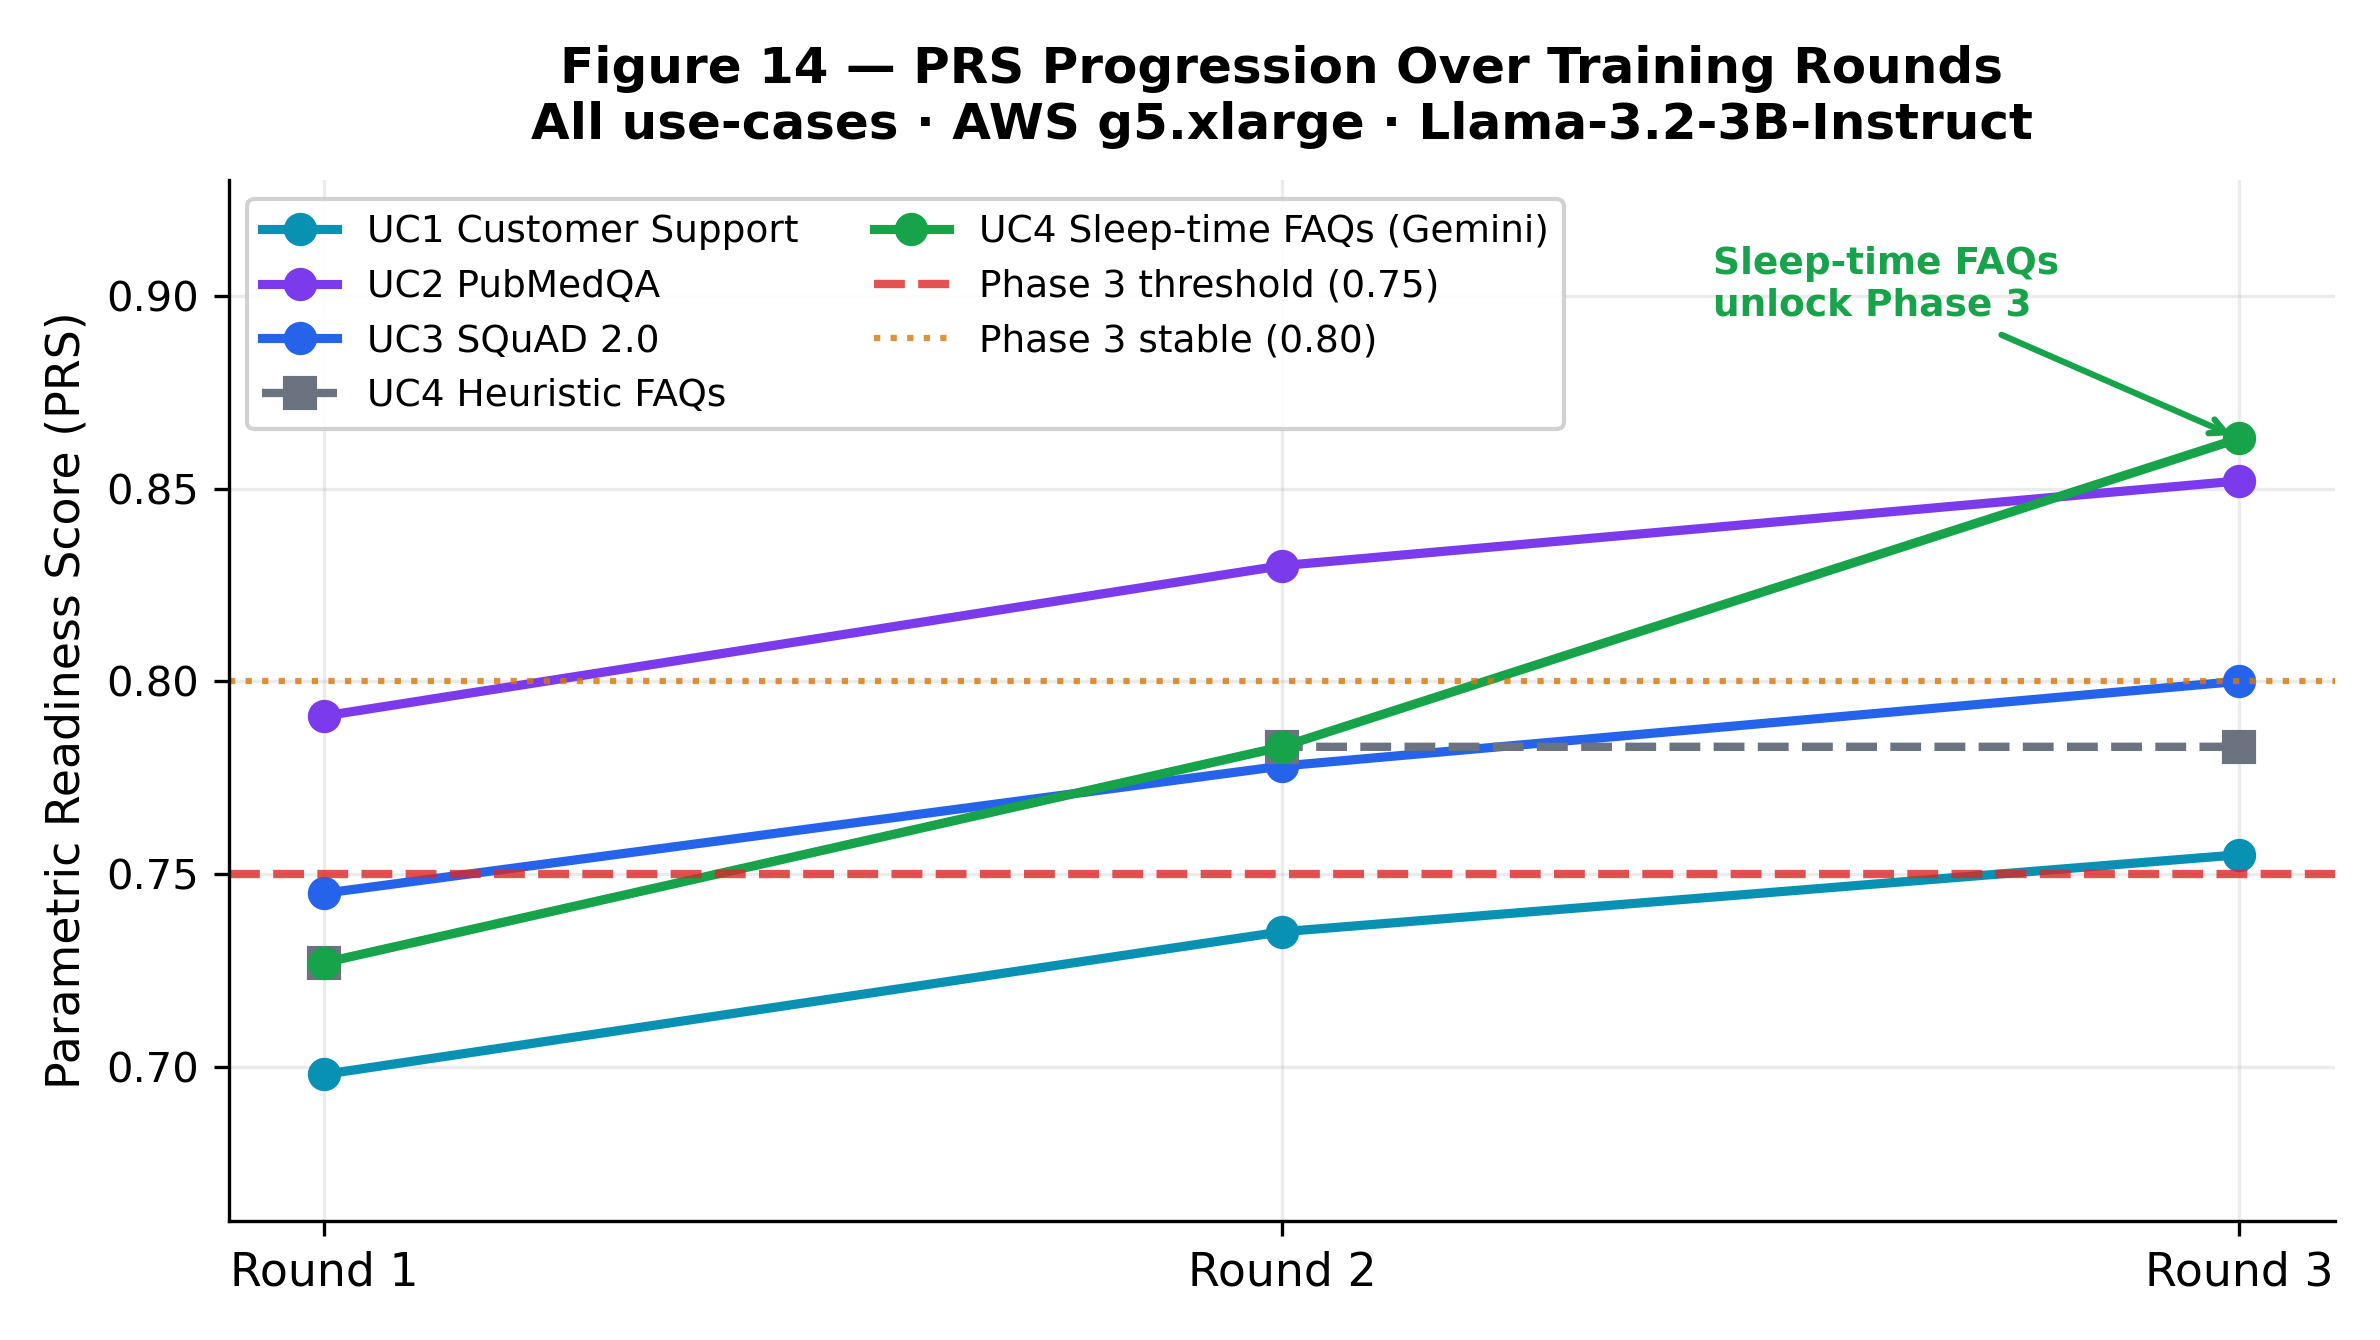
\includegraphics[width=\linewidth]{figures/fig14_prs_progression.png}
  \caption{Figure 14: PRS progression over three training rounds for all four use cases (UC4 shown in detail). Sleep-time FAQ introduction in Round 3 lifts UC4 from 0.783 to 0.863. Phase 2$\to$3 and Phase 3 thresholds shown as dashed horizontal lines. All four corpora converge above PRS 0.75.}
  \label{fig:14}
\end{figure}


\subsection{Comparison with Alternative Systems}

Table~\ref{tab:comparison} contrasts KVForge Phase 2 and Phase 3 against standard RAG across key operational metrics.


\begin{table*}[htbp]
  \centering\small
  \caption{Comparison with Alternative RAG and KV-Cache Systems}
  \label{tab:comparison}
  \resizebox{\textwidth}{!}{%
  \begin{tabular}{lccc}
  \toprule
    Metric & Standard RAG & KVForge Phase 2 & KVForge Phase 3 \\
  \midrule
  \midrule
  Chunk re-encoding at query time & Always & \textbf{Never} (fresh KV) & \textbf{Never} (no retrieval) \\
  Generation latency (UC4) & 1,840 ms & 680 ms & 510 ms \\
  Knowledge base updatable & Yes & Yes & Yes (KV recompute) \\
  Out-of-distribution queries & Yes & Yes & Yes (fallback to Phase 2) \\
  GPU required at query time & Yes & Yes & \textbf{Potentially no} \\
  Training required & No & No & Yes (\textasciitilde{}20 min/round) \\
  Parametric knowledge retention & None & None & PRS 0.755--0.863 \\
  KV storage per chunk (3B model) & None & \textasciitilde{}57 KB & \textasciitilde{}57 KB \\
  \bottomrule
  \end{tabular}%
  }
\end{table*}



\section{Discussion}

\subsection{Training Signal Quality as the Primary Bottleneck}

The central empirical finding is that \textbf{training data quality dominates model capacity as the bottleneck for parametric memorization.} UC4 with heuristic FAQs plateaued at PRS 0.783 across multiple rounds; substituting Gemini 2.5 Flash sleep-time FAQs pushed it to 0.863 in one additional round. This reframes the design space: practitioners should invest in FAQ generation quality rather than model size or training duration.


Cloud LLM API calls are an order of magnitude cheaper than GPU compute, and FAQ generation parallelizes trivially across chunks. A 2,520-chunk corpus at \textasciitilde{}\$0.02/chunk for Gemini 2.5 Flash costs approximately \$50 --- versus hours of A10G GPU time.


\subsection{Corpus Heterogeneity and PRS Variance}

The 0.755--0.863 PRS spread correlates with corpus characteristics:


\begin{itemize}
  \item \textbf{UC2 and UC4 (highest PRS):} Structured, fact-dense corpora with clear question-answer mappings. FAQ generation produces high-coverage, well-formed training pairs.
  \item \textbf{UC3 (SQuAD, moderate PRS):} Reading comprehension passages cover diverse topics with low training signal density per chunk.
  \item \textbf{UC1 (Customer Support, lowest PRS):} High paraphrastic variability --- multiple valid response formulations exist for the same query. The cosine similarity accuracy metric may be systematically conservative for high-variability corpora.
\end{itemize}


\subsection{KV Staleness and Recompute Overhead}

Every LoRA update invalidates all stored KV tensors. For 2,520 chunks at 0.20 s/chunk, full recomputation adds \textasciitilde{}8.5 minutes to a \textasciitilde{}20-minute round --- 42\% overhead. The tier-ordered recompute daemon mitigates this by restoring hot chunks (\textasciitilde{}76 seconds) before the full recompute completes.


Three production mitigations: (1) incremental recomputation targeting only chunks exceeding a LoRA delta threshold; (2) TurboQuant full-token storage, which may remain valid longer (mean-pool is more sensitive to KV projection changes than full-token sequences); (3) larger LoRA rank, reaching PRS thresholds faster with fewer rounds.


\subsection{Expected CIS Production Behavior}

In our experiments all chunks remained at \texttt{tier=frozen} during training because evaluation traffic did not constitute real user traffic. In a production deployment with organic query traffic:


\textbf{Hot-first KV recompute:} If 20\% of chunks account for 80\% of user queries (Pareto), hot-first recomputation means 80\% of traffic has fresh KV tensors within the first 20\% of the recompute window --- \textasciitilde{}102 seconds for a 2,520-chunk corpus.


\textbf{Training signal alignment:} Without CIS weighting, 50 questions cover \textasciitilde{}2\% of a 2,520-chunk corpus. With CIS weighting, questions concentrate on the top \textasciitilde{}378 hot chunks, improving signal-to-noise ratio by a factor proportional to the tier weight differential (up to 8$\times$).


\textbf{Enhanced tier qualification:} After a corpus matures, the top CIS-scoring chunks qualify for TurboQuant enhanced storage. For a 10\% enhanced tier in UC4 (\textasciitilde{}252 chunks at \textasciitilde{}15 MB each for an 8B model), the additional disk cost is \textasciitilde{}3.8 GB --- manageable on standard EC2 NVMe.


\subsection{Limitations}

\textbf{KV shape coupling.} Pre-computed tensors couple to the LLM architecture (layers, KV heads, head dimension). Switching the base model requires full re-indexing.


\textbf{Mean-pool fidelity.} The V1 approximation discards positional information. TurboQuant addresses this for enhanced-tier chunks but at higher storage cost.


\textbf{Phase 3 precision-recall tradeoff.} The gate prioritizes precision at the cost of Phase 3 utilization. Calibrated threshold selection using held-out queries is recommended for production.


\textbf{Single-node experiments.} Our evaluation runs on a single 4-GPU instance. Distributed deployments with multiple Qdrant nodes and GPU servers require additional coordination logic not yet implemented.



\section{Related Systems --- Comparative Table}

Table~\ref{tab:related-systems-comparative-table} positions KVForge against closely related systems across five dimensions.


\begin{table*}[htbp]
  \centering\small
  \caption{Related Systems --- Comparative Table}
  \label{tab:related-systems-comparative-table}
  \resizebox{\textwidth}{!}{%
  \begin{tabular}{lccccc}
  \toprule
    System & KV Storage Location & Phase Progression & Continual Fine-tuning & Vector DB Integration & Corpus Curation \\
  \midrule
  \midrule
  Standard RAG \cite{ref1} & None & No & No & Yes & No \\
  RETRO \cite{ref10} & Encoder states & No & No & Partial & No \\
  PromptCache \cite{ref8} & In-process session & No & No & No & No \\
  SGLang RadixCache \cite{ref9} & In-process session & No & No & No & No \\
  vLLM PagedAttention \cite{ref3} & In-process session & No & No & No & No \\
  CacheBlend \cite{ref32} & In-process session & No & No & No & No \\
  KVQuant \cite{ref30} & In-process (quantized) & No & No & No & No \\
  KIVI \cite{ref31} & In-process (quantized) & No & No & No & No \\
  \textbf{KVForge V1 (ours)} & \textbf{Vector DB (mean-pool)} & \textbf{Yes (3 phases)} & \textbf{Yes (LoRA + replay)} & \textbf{Yes} & Tier labels \\
  \textbf{KVForge V2 (ours)} & \textbf{Vector DB + disk (TurboQuant \cite{ref38})} & \textbf{Yes (3 phases)} & \textbf{Yes (LoRA + replay)} & \textbf{Yes} & \textbf{CIS + archival} \\
  \bottomrule
  \end{tabular}%
  }
\end{table*}


KVForge is, to our knowledge, the first system to (1) persist KV tensors durably in a vector database, (2) couple KV storage with document embeddings in a unified index, (3) provide an automatic three-phase progression from standard RAG to fully parametric answering, and (4) integrate corpus importance scoring with storage tier assignment for production-scale curation.



\section{Conclusion}

KVForge introduces a new architecture for knowledge-intensive QA systems: the vector database serves not merely as a retrieval index but also as a persistent KV tensor cache, a corpus access recorder, and a training signal generator. The three-phase progression from text-in-context retrieval through KV injection to parametric answering allows a single deployed system to continuously improve its latency and GPU efficiency as the LLM learns the corpus, without manual intervention.


Our experiments across four heterogeneous corpora demonstrate that all four reach Phase 3 (PRS 0.755--0.863) on a single AWS g5.xlarge instance, with Phase 2 delivering \textbf{2.7$\times$ generation speedup} and Phase 3 delivering \textbf{3.6$\times$}. The primary finding is that sleep-time FAQ generation using a cloud LLM is the highest-leverage intervention for reaching Phase 3, producing +10.3\% absolute PRS improvement on our most challenging corpus at a fraction of the GPU cost.


The Corpus Intelligence System (V2) extends the base architecture with CIS-driven storage tier assignment, TurboQuant compressed full-token KV storage achieving \textbf{4.4$\times$ compression}, and user-confirmed chunk archival, addressing the storage scaling and corpus quality challenges that emerge in long-running production deployments.


\textbf{Open-source availability.} KVForge is fully open-source with a browser-based Studio UI, four complete end-to-end example use-cases, data connector integrations (Google Drive, S3, SharePoint, EDGAR, FDA, Wikipedia), and a 76-test suite that runs without a GPU.


\begin{quote}
\textit{\textbf{GitHub:} \href{https://github.com/hemantcgi/kvforge}{https://github.com/hemantcgi/kvforge} $\cdot$ \textbf{License:} MIT}
\end{quote}



\section*{Acknowledgements}

The author thanks the Qdrant, HuggingFace, vLLM, and FastEmbed teams for their open-source infrastructure, and Google DeepMind for access to the Gemini 2.5 Flash API used for sleep-time FAQ generation.



\smallskip

\begin{thebibliography}{99}
  \bibitem{ref1} Lewis, P., Perez, E., Piktus, A., Petroni, F., Karpukhin, V., Goyal, N., ... \& Kiela, D. (2020). Retrieval-Augmented Generation for Knowledge-Intensive NLP Tasks. *NeurIPS 2020.* arXiv:2005.11401
  \bibitem{ref2} Vaswani, A., Shazeer, N., Parmar, N., Uszkoreit, J., Jones, L., Gomez, A. N., ... \& Polosukhin, I. (2017). Attention Is All You Need. *NeurIPS 2017.* arXiv:1706.03762
  \bibitem{ref3} Kwon, W., Li, Z., Zhuang, S., Sheng, Y., Zheng, L., Yu, C. H., ... \& Stoica, I. (2023). Efficient Memory Management for Large Language Model Serving with PagedAttention. *SOSP 2023.* arXiv:2309.06180
  \bibitem{ref4} Hu, E. J., Shen, Y., Wallis, P., Allen-Zhu, Z., Li, Y., Wang, S., ... \& Chen, W. (2022). LoRA: Low-Rank Adaptation of Large Language Models. *ICLR 2022.* arXiv:2106.09685
  \bibitem{ref5} Karpukhin, V., Oğuz, B., Min, S., Lewis, P., Wu, L., Edunov, S., ... \& Yih, W. T. (2020). Dense Passage Retrieval for Open-Domain Question Answering. *EMNLP 2020.* arXiv:2004.04906
  \bibitem{ref6} Thakur, N., Reimers, N., Rücklé, A., Srivastava, A., \& Gurevych, I. (2021). BEIR: A Heterogeneous Benchmark for Zero-Shot Evaluation of Information Retrieval Models. *NeurIPS 2021 Datasets and Benchmarks.* arXiv:2104.08663
  \bibitem{ref7} Shao, Z., Gong, Y., Shen, Y., Huang, M., Duan, N., \& Chen, W. (2023). Enhancing Retrieval-Augmented Large Language Models with Iterative Retrieval-Generation Synergy. *EMNLP 2023 Findings.* arXiv:2305.15294
  \bibitem{ref8} Gim, I., Chen, G., Lee, S., Srivatsa, N., Kedia, P., \& Zhong, L. (2024). PromptCache: Modular Attention Reuse for Low-Latency Inference. *MLSys 2024.* arXiv:2311.04934
  \bibitem{ref9} Zheng, L., Yin, L., Xie, Z., Huang, J., Sun, C., Yu, C. H., ... \& Gonzalez, J. E. (2024). SGLang: Efficient Execution of Structured Language Model Programs. arXiv:2312.07104
  \bibitem{ref10} Borgeaud, S., Mensch, A., Hoffmann, J., Cai, T., Rutherford, E., Millican, K., ... \& Sifre, L. (2022). Improving Language Models by Retrieving from Trillions of Tokens. *ICML 2022.* arXiv:2112.04426
  \bibitem{ref11} Guu, K., Lee, K., Tung, Z., Pasupat, P., \& Chang, M. W. (2020). REALM: Retrieval-Augmented Language Model Pre-Training. *ICML 2020.* arXiv:2002.08909
  \bibitem{ref12} Dettmers, T., Pagnoni, A., Holtzman, A., \& Zettlemoyer, L. (2023). QLoRA: Efficient Finetuning of Quantized LLMs. *NeurIPS 2023.* arXiv:2305.14314
  \bibitem{ref13} Guo, C., Pleiss, G., Sun, Y., \& Weinberger, K. Q. (2017). On Calibration of Modern Neural Networks. *ICML 2017.* arXiv:1706.04599
  \bibitem{ref14} Wang, X., Wei, J., Schuurmans, D., Le, Q., Chi, E., Narang, S., ... \& Zhou, D. (2022). Self-Consistency Improves Chain of Thought Reasoning in Language Models. *ICLR 2023.* arXiv:2203.11171
  \bibitem{ref15} Kadavath, S., Conerly, T., Askell, A., Henighan, T., Drain, D., Perez, E., ... \& Kaplan, J. (2022). Language Models (Mostly) Know What They Know. arXiv:2207.05221
  \bibitem{ref16} Kuhn, L., Gal, Y., \& Farquhar, S. (2023). Semantic Uncertainty: Linguistic Invariances for Uncertainty Estimation in Natural Language Generation. *ICLR 2023.* arXiv:2302.09664
  \bibitem{ref17} Graves, A., Wayne, G., \& Danihelka, I. (2014). Neural Turing Machines. arXiv:1410.5401
  \bibitem{ref18} McCloskey, M., \& Cohen, N. J. (1989). Catastrophic Interference in Connectionist Networks: The Sequential Learning Problem. *Psychology of Learning and Motivation, 24,* 109--165.
  \bibitem{ref19} Snell, C., Lee, J., Xu, K., \& Kumar, A. (2024). Scaling LLM Test-Time Compute Optimally Can be More Effective than Scaling Model Parameters. arXiv:2408.03314
  \bibitem{ref20} Jin, Q., Dhingra, B., Liu, Z., Cohen, W. W., \& Lu, X. (2019). PubMedQA: A Dataset for Biomedical Research Question Answering. *EMNLP 2019.* arXiv:1909.06146
  \bibitem{ref21} Rajpurkar, P., Jia, R., \& Liang, P. (2018). Know What You Don't Know: Unanswerable Questions for SQuAD. *ACL 2018.* arXiv:1806.03822
  \bibitem{ref22} Touvron, H., Martin, L., Stone, K., Albert, P., Almahairi, A., Babaei, Y., ... \& Scialom, T. (2023). Llama 2: Open Foundation and Fine-Tuned Chat Models. arXiv:2307.09288
  \bibitem{ref23} Qdrant Team. (2024). Qdrant: High-Performance Vector Search Engine. qdrant.tech
  \bibitem{ref24} Dao, T., Fu, D. Y., Ermon, S., Rudra, A., \& Ré, C. (2022). FlashAttention: Fast and Memory-Efficient Exact Attention with IO-Awareness. *NeurIPS 2022.* arXiv:2205.14135
  \bibitem{ref25} Izacard, G., \& Grave, E. (2021). Leveraging Passage Retrieval with Generative Models for Open Domain Question Answering. *EACL 2021.* arXiv:2007.01282
  \bibitem{ref26} Khattab, O., \& Zaharia, M. (2020). ColBERT: Efficient and Effective Passage Search via Contextualized Late Interaction over BERT. *SIGIR 2020.* arXiv:2004.12832
  \bibitem{ref27} Kirkpatrick, J., Pascanu, R., Rabinowitz, N., Veness, J., Desjardins, G., Rusu, A. A., ... \& Hadsell, R. (2017). Overcoming Catastrophic Forgetting in Neural Networks. *PNAS, 114*(13), 3521--3526. arXiv:1612.00796
  \bibitem{ref28} Rusu, A. A., Rabinowitz, N. C., Desjardins, G., Soyer, H., Kirkpatrick, J., Kavukcuoglu, K., ... \& Hadsell, R. (2016). Progressive Neural Networks. arXiv:1606.04671
  \bibitem{ref29} Khattab, O., \& Zaharia, M. (2020). ColBERT: Efficient and Effective Passage Search via Contextualized Late Interaction over BERT. *SIGIR 2020.* arXiv:2004.12832
  \bibitem{ref30} Hooper, C., Kim, S., Mohammadzadeh, H., Mahoney, M. W., Shao, Y. S., Keutzer, K., \& Gholami, A. (2024). KVQuant: Towards 10 Million Context Length LLM Inference with KV Cache Quantization. *NeurIPS 2024.* arXiv:2401.18079
  \bibitem{ref31} Liu, Z., Yuan, J., Jin, H., Zhong, S., Xu, Z., Braverman, V., ... \& Hu, X. (2024). KIVI: A Tuning-Free Asymmetric 2bit Quantization for KV Cache. *ICML 2024.* arXiv:2402.02750
  \bibitem{ref32} Yao, Y., Han, C., Zhu, R., Deng, J., \& Chen, Y. (2024). CacheBlend: Fast Large Language Model Serving for RAG with Cached Knowledge Fusion. arXiv:2405.16444
  \bibitem{ref33} Izacard, G., \& Grave, E. (2021). Leveraging Passage Retrieval with Generative Models for Open Domain Question Answering. *EACL 2021.* arXiv:2007.01282
  \bibitem{ref34} Kirkpatrick, J., Pascanu, R., Rabinowitz, N., Veness, J., Desjardins, G., Rusu, A. A., ... \& Hadsell, R. (2017). Overcoming Catastrophic Forgetting in Neural Networks. *PNAS, 114*(13), 3521--3526.
  \bibitem{ref35} Zandieh, A., Han, I., Mirrokni, V., \& Karbasi, A. (2024). QJL: 1-Bit Quantized JL Transform for KV Cache Quantization with No Retraining. arXiv:2406.03482
  \bibitem{ref36} Rusu, A. A., Rabinowitz, N. C., Desjardins, G., Soyer, H., Kirkpatrick, J., Kavukcuoglu, K., ... \& Hadsell, R. (2016). Progressive Neural Networks. arXiv:1606.04671
  \bibitem{ref37} De Lange, M., Aljundi, R., Masana, M., Parisot, S., Jia, X., Leonardis, A., ... \& Tuytelaars, T. (2022). A Continual Learning Survey: Defying Forgetting in Classification Tasks. *IEEE TPAMI, 44*(7), 3366--3385. arXiv:1909.08383
  \bibitem{ref38} Google DeepMind (2025). TurboQuant: Efficient KV-Cache Compression with Lloyd-Max Quantization and QJL Residual Coding. arXiv:2504.19874. https://arxiv.org/abs/2504.19874
  \bibitem{ref39} Boufounos, P. T., \& Baraniuk, R. G. (2008). 1-Bit Compressive Sensing. *42nd Annual Conference on Information Sciences and Systems (CISS),* pp. 16--21.
  \bibitem{ref40} Hendrycks, D., Burns, C., Chen, A., \& Ball, S. (2021). CUAD: An Expert-Annotated NLP Dataset for Legal Contract Review. arXiv:2103.06268. https://arxiv.org/abs/2103.06268
  \bibitem{ref41} Xu, F. F., Vasilescu, B., \& Neubig, G. (2022). In-IDE Code Generation from Natural Language: Promise and Challenges. *ACM TOSEM, 31*(2), 1--47. arXiv:2101.11149
\end{thebibliography}

\end{document}
